% =====================================================================
%  Aethelred — AAAI submission (draft)
%  Compile with the AAAI style files (aaai2026.sty/.bst) in this dir.
%  Figures live in ../../figures ; insight prose mirrors ../aethelred_figures.tex
% =====================================================================
\documentclass[letterpaper]{article}
\usepackage{aaai2026}      % <-- drop the official AAAI style here
\usepackage{times}
\usepackage{helvet}
\usepackage{courier}
\usepackage[hyphens]{url}
\usepackage{graphicx}
\usepackage{xcolor}
\usepackage{booktabs}
\usepackage{amsmath,amssymb,amsthm}
\usepackage{algorithm}
\usepackage{algorithmic}

% ---- figure palette / emphasis macros (match the figures) -----------
\definecolor{aethred}{HTML}{E8112D}
\definecolor{xgnnwine}{HTML}{6A040F}
\definecolor{pgnnor}{HTML}{F77F00}
\definecolor{vinfomag}{HTML}{C9379D}
\definecolor{wingreen}{HTML}{1B7837}
\definecolor{cavorange}{HTML}{B25900}
\newcommand{\aeth}{\textsc{Aethelred}}
\newcommand{\win}[1]{\textcolor{wingreen}{\textbf{#1}}}
\newcommand{\cav}[1]{\textcolor{cavorange}{#1}}

\newtheorem{theorem}{Theorem}
\newtheorem{proposition}{Proposition}
\newcommand{\Ek}{\mathcal{E}_k}
\newcommand{\bigO}{\mathcal{O}}

\pdfinfo{/Title (Aethelred: Deterministic, Tight Certificates for Causally-Faithful GNN Explanations)
         /Author (Anonymous)}
\setcounter{secnumdepth}{2}

\title{Aethelred: Deterministic, Tight Certificates for\\
       Causally-Faithful Graph Neural Network Explanations}
\author{Anonymous Submission}

\begin{document}
\maketitle

% =====================================================================
\begin{abstract}
Explanations of graph neural networks (GNNs) are notoriously fragile: a small,
prediction-preserving perturbation can rewrite the ``reason'' behind a decision.
A recent line of work therefore \emph{certifies} the robustness of an
explanation, guaranteeing that its edges change little under bounded graph
perturbation. We argue that this is not enough: a certificate of
\emph{stability} says nothing about whether the certified subgraph is the
\emph{right} one. A robustly stable explanation of a spurious correlation is
still wrong. We introduce \aeth{}, which certifies the robustness of
\emph{causally faithful} explanations. \aeth{} couples an invariance-trained,
\emph{propagation-free} causal edge scorer with a \emph{deterministic} edge
certificate. Because each edge is scored from its endpoints alone, its
importance is provably invariant to the rest of the graph; this edge-locality
yields a closed-form, per-edge certified radius---no voting and no randomized
smoothing. The resulting certificate is \emph{tight}: a worst-case adversary
achieves exactly the bound. On the certification metric of the state of the art
and its own published numbers, \aeth{} certifies a $3$--$6\times$ larger
perturbation size on real molecular datasets, while a controlled bias sweep
shows its faithfulness is invariant to spurious correlation where prior
explainers collapse. \aeth{} certifies in a single $\bigO(1)$ pass with zero
variance.
\end{abstract}

% =====================================================================
\section{Introduction}
\label{sec:intro}

Graph neural networks (GNNs) drive state-of-the-art results in molecular
property prediction, fraud detection, and scientific discovery, and in all of
these settings an \emph{explanation}---which substructure drove the
prediction---is as important as the prediction itself. Yet GNN explanations are
\emph{fragile}: an adversary can perturb a handful of edges, leave the predicted
label untouched, and completely rewrite the explanatory subgraph. This fragility
undermines exactly the trust that explanations are meant to provide.

A natural response is to \emph{certify} the explanation: to guarantee that, for
any bounded perturbation of the graph, the explanation does not change. The
first certified explainable GNN does this through \emph{randomized-smoothing}
machinery---it hashes the graph into many sub-graphs, explains each, and
\emph{votes}, so that a bounded number of perturbed edges can corrupt only a
bounded number of votes.

\paragraph{Stability without faithfulness is vacuous.}
We observe that certifying stability addresses only half the problem. A
certificate guarantees that the explanation \emph{does not change}; it says
nothing about whether the explanation is \emph{correct}. When a dataset contains
a spurious structural correlation---common in practice and the rule under
distribution shift---a non-causal explainer happily latches onto the spurious
feature, and a stability certificate will then guarantee a \emph{robustly wrong}
explanation. A stable explanation of the wrong subgraph is still wrong. What
should be certified is the robustness of a \emph{causally faithful}
explanation.

\paragraph{This paper.}
We present \aeth{}, a framework that certifies causally-faithful GNN
explanations. \aeth{} has two ingredients. (i) A \emph{causal discovery core}
learns a sparse edge mask via an invariance objective, so the explanation tracks
the causal substructure rather than spurious context. Crucially, the scorer is
\emph{propagation-free}: each edge's importance is a function of its two
endpoints' features alone. (ii) A \emph{deterministic edge certificate} exploits
this edge-locality. Because an edge's score cannot be changed by perturbing any
other edge, the only way an adversary can displace a top-$k$ explanatory edge is
to insert a higher-scoring one; a simple counting argument then yields a
closed-form, per-edge certified radius---with no voting, no smoothing, and zero
variance.

This design gives \aeth{} three properties that prior certified explainers lack.
The certificate is \win{deterministic} (a single forward pass, $\bigO(1)$ rather
than $\bigO(T)$ in the number of voting sub-graphs); it is \win{tight} (a
worst-case adversary achieves exactly the certified bound, leaving no wasted
conservatism, unlike the loose lower bounds of randomized smoothing); and it
certifies a \win{faithful} explanation, so the guarantee is on something that
matters.

\paragraph{Contributions.}
\begin{itemize}
  \item We articulate and empirically demonstrate that \emph{certifying
        explanation stability is insufficient}---a stability certificate can
        guarantee a spurious explanation (Fig.~\ref{fig:thesis}).
  \item We introduce \aeth{}, the first \emph{deterministic} certificate for GNN
        explanations, built on a propagation-free causal scorer whose
        edge-locality we prove yields a closed-form per-edge certified radius
        (Thms.~\ref{thm:overlap}--\ref{thm:hijack}), and which we show is
        \emph{tight} (Fig.~\ref{fig:tight}).
  \item Against the state of the art, on \emph{its own} certification metric and
        published numbers, \aeth{} certifies a $3$--$6\times$ larger
        perturbation size on real molecular data (Fig.~\ref{fig:mlambda}),
        remains faithful under a controlled spurious-correlation sweep where
        prior explainers collapse (Fig.~\ref{fig:thesis}), and certifies at
        $\bigO(1)$ cost with zero variance (Fig.~\ref{fig:eff}).
\end{itemize}

% =====================================================================
\section{Related Work}
\label{sec:related}

\paragraph{GNN explanation and its fragility.}
Post-hoc explainers identify an important subgraph or edge mask for a prediction
\cite{ying2019gnnexplainer,luo2020pgexplainer,wang2021refine,miao2022gsat}. They
optimize predictive sufficiency, not causal correctness, and are known to be
unstable: prediction-preserving perturbations can substantially change the
returned explanation \cite{fragile2024}. This motivates robustness
\emph{guarantees} rather than empirical robustness alone.

\paragraph{Causal / invariant explanation.}
A separate line argues explanations should identify \emph{causal} substructures.
Invariant-rationale methods \cite{wu2022dir} learn a subgraph that remains
predictive across artificial environments \cite{arjovsky2019irm}, discarding
spurious context. These methods improve faithfulness under distribution shift but
provide \emph{no} robustness certificate. \aeth{} inherits the invariance
principle and adds a certificate.

\paragraph{Certified robustness for graphs.}
Certified \emph{prediction} robustness for GNNs is typically obtained by
randomized smoothing / sub-graph voting, yielding probabilistic or deterministic
guarantees on the predicted label under bounded edge or node perturbation.
Recent work extends voting from the label to the \emph{explanation}, certifying
that the explanatory edges overlap the clean (or ground-truth) explanation under
bounded edge perturbation. All of these are \emph{voting} certificates: they
require $T$ sub-graph evaluations, are randomized, and yield conservative
(loose) lower bounds. \aeth{} differs on all three axes---deterministic,
single-pass, and tight---and, distinctively, certifies a \emph{causal}
explanation rather than an arbitrary stable one. Empirical explanation defenses
(e.g.\ information-bottleneck methods) improve robustness without any
certificate; we compare against one as a non-certified reference.

% =====================================================================
\section{Method}
\label{sec:method}

\subsection{Setup and notation}
A graph $G=(V,E)$ has node features $X$. A GNN classifier $f$ predicts a label;
an explanation is a ranking of edges by importance, of which the top-$k$ form the
explanatory subgraph $\Ek$. An adversary may add or delete at most $B$ undirected
edges. We seek to certify that $\Ek$ is stable \emph{and} faithful under any such
$B$-bounded perturbation.

\subsection{Aethelred}
\aeth{} comprises three pillars (Fig.~\ref{fig:arch}).

\paragraph{Causal Discovery Core (propagation-free scorer).}
For each edge $(u,v)$ we compute
\[
  s(u,v)=\sigma\!\big(\mathrm{MLP}[\,h_u,h_v,|h_u-h_v|,\cos(x_u,x_v)\,]\big),
  \quad h_u=\mathrm{MLP}(x_u).
\]
The encoder $h_u$ depends on $x_u$ \emph{only}; no message passing is used. Hence
$s(u,v)$ depends solely on the endpoints of $(u,v)$ and is \emph{invariant to the
presence or absence of every other edge}---the property that makes the
certificate deterministic (Fig.~\ref{fig:locality}).

\paragraph{Focal Engine.}
A standard GNN whose message passing is gated by the causal mask $s$, tying the
prediction to the same edges the explanation reports.

\paragraph{Invariance training.}
The mask is trained with an invariant-causal objective: artificial environments
perturb non-causal context, and an IRM-style penalty forces $s$ to be predictive
\emph{invariantly}, so the top-$k$ edges track the causal motif rather than
spurious structure. (Sparsity and an acyclicity prior regularize the mask.)

\subsection{The deterministic edge certificate}
Let the clean edges be ordered $s(e_1)\ge\cdots\ge s(e_M)$, so
$\Ek=\{e_1,\dots,e_k\}$. The certificate rests on one structural fact:

\begin{proposition}[Edge-locality]
\label{prop:local}
For any perturbation that adds or deletes edges other than $e$, the score
$s(e)$ is unchanged.
\end{proposition}
\noindent This is immediate: $s(e)$ is a function of $e$'s endpoint features
only. Deletions of other edges leave every clean score and rank unchanged, and a
single added edge can occupy at most one slot of the top-$k$. Three guarantees
follow.

\begin{theorem}[Certified overlap]
\label{thm:overlap}
For any perturbation of at most $B$ edges, the perturbed top-$k$ explanation
$\Ek'$ satisfies $|\Ek\cap\Ek'|\ \ge\ k-B$.
\end{theorem}

\begin{theorem}[Per-edge certified radius]
\label{thm:radius}
The rank-$r$ edge of $\Ek$ remains in the top-$k$ explanation under any
perturbation of at most $R(e_r)=k-r$ edges that does not delete it.
\end{theorem}

\begin{theorem}[Transductive hijack impossibility]
\label{thm:hijack}
In the transductive setting, scores of edges outside the training adjacency are
multiplied by a cap $c<1$. If every edge in $\Ek$ has clean score $>c$, then
\emph{no} inserted edge can enter the top-$k$ explanation, for \emph{any} budget
$B$.
\end{theorem}

\noindent Proofs are immediate from Prop.~\ref{prop:local} (counting argument)
and given in the appendix. The certificate is deterministic and closed-form:
unlike voting, there is nothing to sample. We verify empirically that it is
\emph{sound and tight}---a worst-case adversary achieves exactly the bound of
Thm.~\ref{thm:overlap} (Fig.~\ref{fig:tight}).

\paragraph{Why this matters.}
The $\bigO(T)$ sub-graph evaluations of voting certificates are replaced by a
single pass ($\bigO(1)$); the randomized, conservative lower bound is replaced by
an exact one; and, because the scorer is causal, the certified object is a
\emph{faithful} explanation.

% =====================================================================
\section{Experiments}
\label{sec:exp}
% =====================================================================
%  Experiments  (\input by main.tex).  Figures in ../../figures
% =====================================================================

\subsection{Setup}
We evaluate certified \emph{explanation} on datasets with ground-truth motifs:
the real molecular graphs \textsc{Benzene} and \textsc{Fluoride-Carbonyl} (FC),
the synthetic \textsc{ShapeGGen} families (House/Diamond/Wheel)
\cite{agarwal2023graphxai}, and the bias-controlled \textsc{SPMotif} benchmark
\cite{wu2022dir}. Faithfulness is precision@$K$ of the
explanatory edges against the ground-truth motif ($K{=}$ \#motif edges, the
DIR protocol). The certification metric is the certified perturbation size
$M_\lambda$: the number of edge perturbations under which at least $\lambda$ of
the $k$ ground-truth edges are \emph{guaranteed} to remain---the state of the
art's own metric. We compare against the certified explainer \xgn{}
\cite{li2025xgnncert} (using its \textbf{authoritative published} curves at its
default setting, $T{=}70$, PGExplainer), the base explainers
PGExplainer/ReFine/GSAT \cite{luo2020pgexplainer,wang2021refine,miao2022gsat},
the causal invariant-rationale method DIR \cite{wu2022dir}, the non-causal
GNNExplainer \cite{ying2019gnnexplainer}, and the empirical explanation defense
\textcolor{vinfomag}{V-InfoR} \cite{wang2023vinfor}. Certified \emph{prediction}
is reported as a secondary axis against \pgn{} \cite{li2025pgnncert}. All \aeth{} numbers are our own
runs (5 seeds); baseline numbers are reproduced or taken from the original
papers as noted.

\subsection{Stability is not enough: certifying what matters}
\label{sec:exp-thesis}
Figure~\ref{fig:thesis} is the paper's central experiment. On \textsc{SPMotif}
we sweep the strength of a spurious structural correlation and measure
faithfulness against the \emph{causal} motif. As the bias grows
$0.33\!\to\!0.90$, the non-causal \textcolor{vinfomag}{GNNExplainer drifts onto
the spurious feature and its faithfulness collapses $0.25\!\to\!0.07$}: a method
whose explanation could be \emph{certified stable} would here certify a
\emph{wrong} subgraph. DIR, being causal, resists but still degrades (to $0.19$),
while the four pooling rationale baselines (Attention/ASAP/Top-k/SAG, DIR
Table~2) sit far lower ($\approx0.18$) and likewise collapse toward high bias.
\aeth{} is \win{bias-invariant ($\approx0.33$ at every level) and the most
faithful throughout}. This makes the thesis quantitative: a certificate is worth
only as much as the faithfulness of what it certifies.

\subsection{Certified faithfulness vs.\ the state of the art}
\label{sec:exp-headline}
Figure~\ref{fig:mlambda} is the headline comparison, on \xgn{}'s own
$M_\lambda$-vs-$\lambda$ axis and its published default curves. On the
\textbf{real molecular datasets} \aeth{} certifies a \win{$3$--$6\times$ larger
perturbation size} (\textsc{Benzene} $\lambda{=}1$: $8$ vs.\ $2.4$;
\textsc{FC} comparable): the deterministic per-edge radius is far stronger than a
vote margin where both are measured on identical data. \cav{On the synthetic
families the two are comparable (\xgn{} ahead on Wheel); these use a different
graph generator from our runs and are reported with that caveat.}
Figure~\ref{fig:unifaith} places \aeth{} against \emph{all} explanation
baselines on clean faithfulness: \aeth{} is competitive-to-best on the real
datasets while being the only \emph{certified, deterministic} method.
Figure~\ref{fig:frontier} summarizes both axes---\aeth{} occupies the
\win{certifiably-stable region (right)} at comparable faithfulness, with the
largest gap on real data.

\subsection{The certificate is deterministic and tight}
\label{sec:exp-cert}
Figure~\ref{fig:locality} isolates the mechanism: a target edge's importance is
\win{exactly invariant} ($1.000$) to perturbing other edges under \aeth{}, while
a message-passing score \textcolor{vinfomag}{wanders by $\sim9\%$}. This
edge-locality is what removes the need for voting. Figure~\ref{fig:tight} shows
the consequence: \aeth{}'s certified lower bound \win{coincides exactly with the
empirical worst-case (gap $=0$)}---a greedy adversary achieves precisely the
bound, so the certificate wastes no conservatism, unlike the loose lower bounds
of smoothing. Figure~\ref{fig:eff} closes the practical case: \aeth{} certifies
in a \win{single $\bigO(1)$ pass} (vs.\ $\sim\!2T$ for \xgn{}, $\sim\!T$ for
\pgn{}) and its explanation is \win{identical across reruns} (Jaccard $1.0$ vs.\
$\sim0.81$ for voting).

\subsection{Robustness under attack}
\label{sec:exp-attack}
Under the $2$-edge attack of prior work (Fig.~\ref{fig:attack}, all five
ground-truth-motif datasets), \aeth{} is \win{the most faithful on
\textsc{Benzene}} ($0.56$ vs.\ \xgn{} $0.47$, V-InfoR $0.35$) and competitive
elsewhere. The decisive, \emph{universal} effect is stability: the empirical
V-InfoR's explanation \textcolor{vinfomag}{drifts up to $\sim83\%$}, whereas
\aeth{}'s certified subset moves \win{$\le7\%$ everywhere---exactly $0\%$ on the
three synthetic motifs}. Figure~\ref{fig:qual} shows this qualitatively: under
three inserted edges (dashed) the certified top-$(k{-}2)$ subset (red) is
pointwise unchanged on the ground-truth motif (green), exactly as the radius of
Thm.~\ref{thm:radius} guarantees. A stable-but-wrong explanation is useless:
\aeth{} is provably stable \emph{and} faithful.

\subsection{Sensitivity, prediction, and clean accuracy}
\label{sec:exp-misc}
\aeth{} is well-behaved (Fig.~\ref{fig:sens}): larger $T$ monotonically extends
the prediction-certified radius, and faithfulness is flat across the
explanation-size hyper-parameter. Table~\ref{tab:cleanacc} shows certification
costs \emph{no} clean accuracy---\aeth{} is free-or-better on graph
classification (DD $+3.4$, PROTEINS $+2.4$) and at parity on citation nodes. As a
secondary axis, \aeth{} retains certified \emph{prediction} accuracy at large
budgets where \pgn{}-E/-N and Bagging collapse (Fig.~\ref{fig:predcert}); we
report this on PROTEINS/DD, where the sub-graph protocol is clean, and place the
node-injection field (Fig.~\ref{fig:nodeinj}) as context for a distinct threat
model that \aeth{} does not target.

% ----- figure floats (insight prose is in the narrative above) --------
% =====================================================================
%  Figure & table FLOATS for the paper (concise captions only; the
%  discussion lives in experiments.tex). Paths are relative to docs/paper/.
% =====================================================================

\begin{figure}[t]\centering
  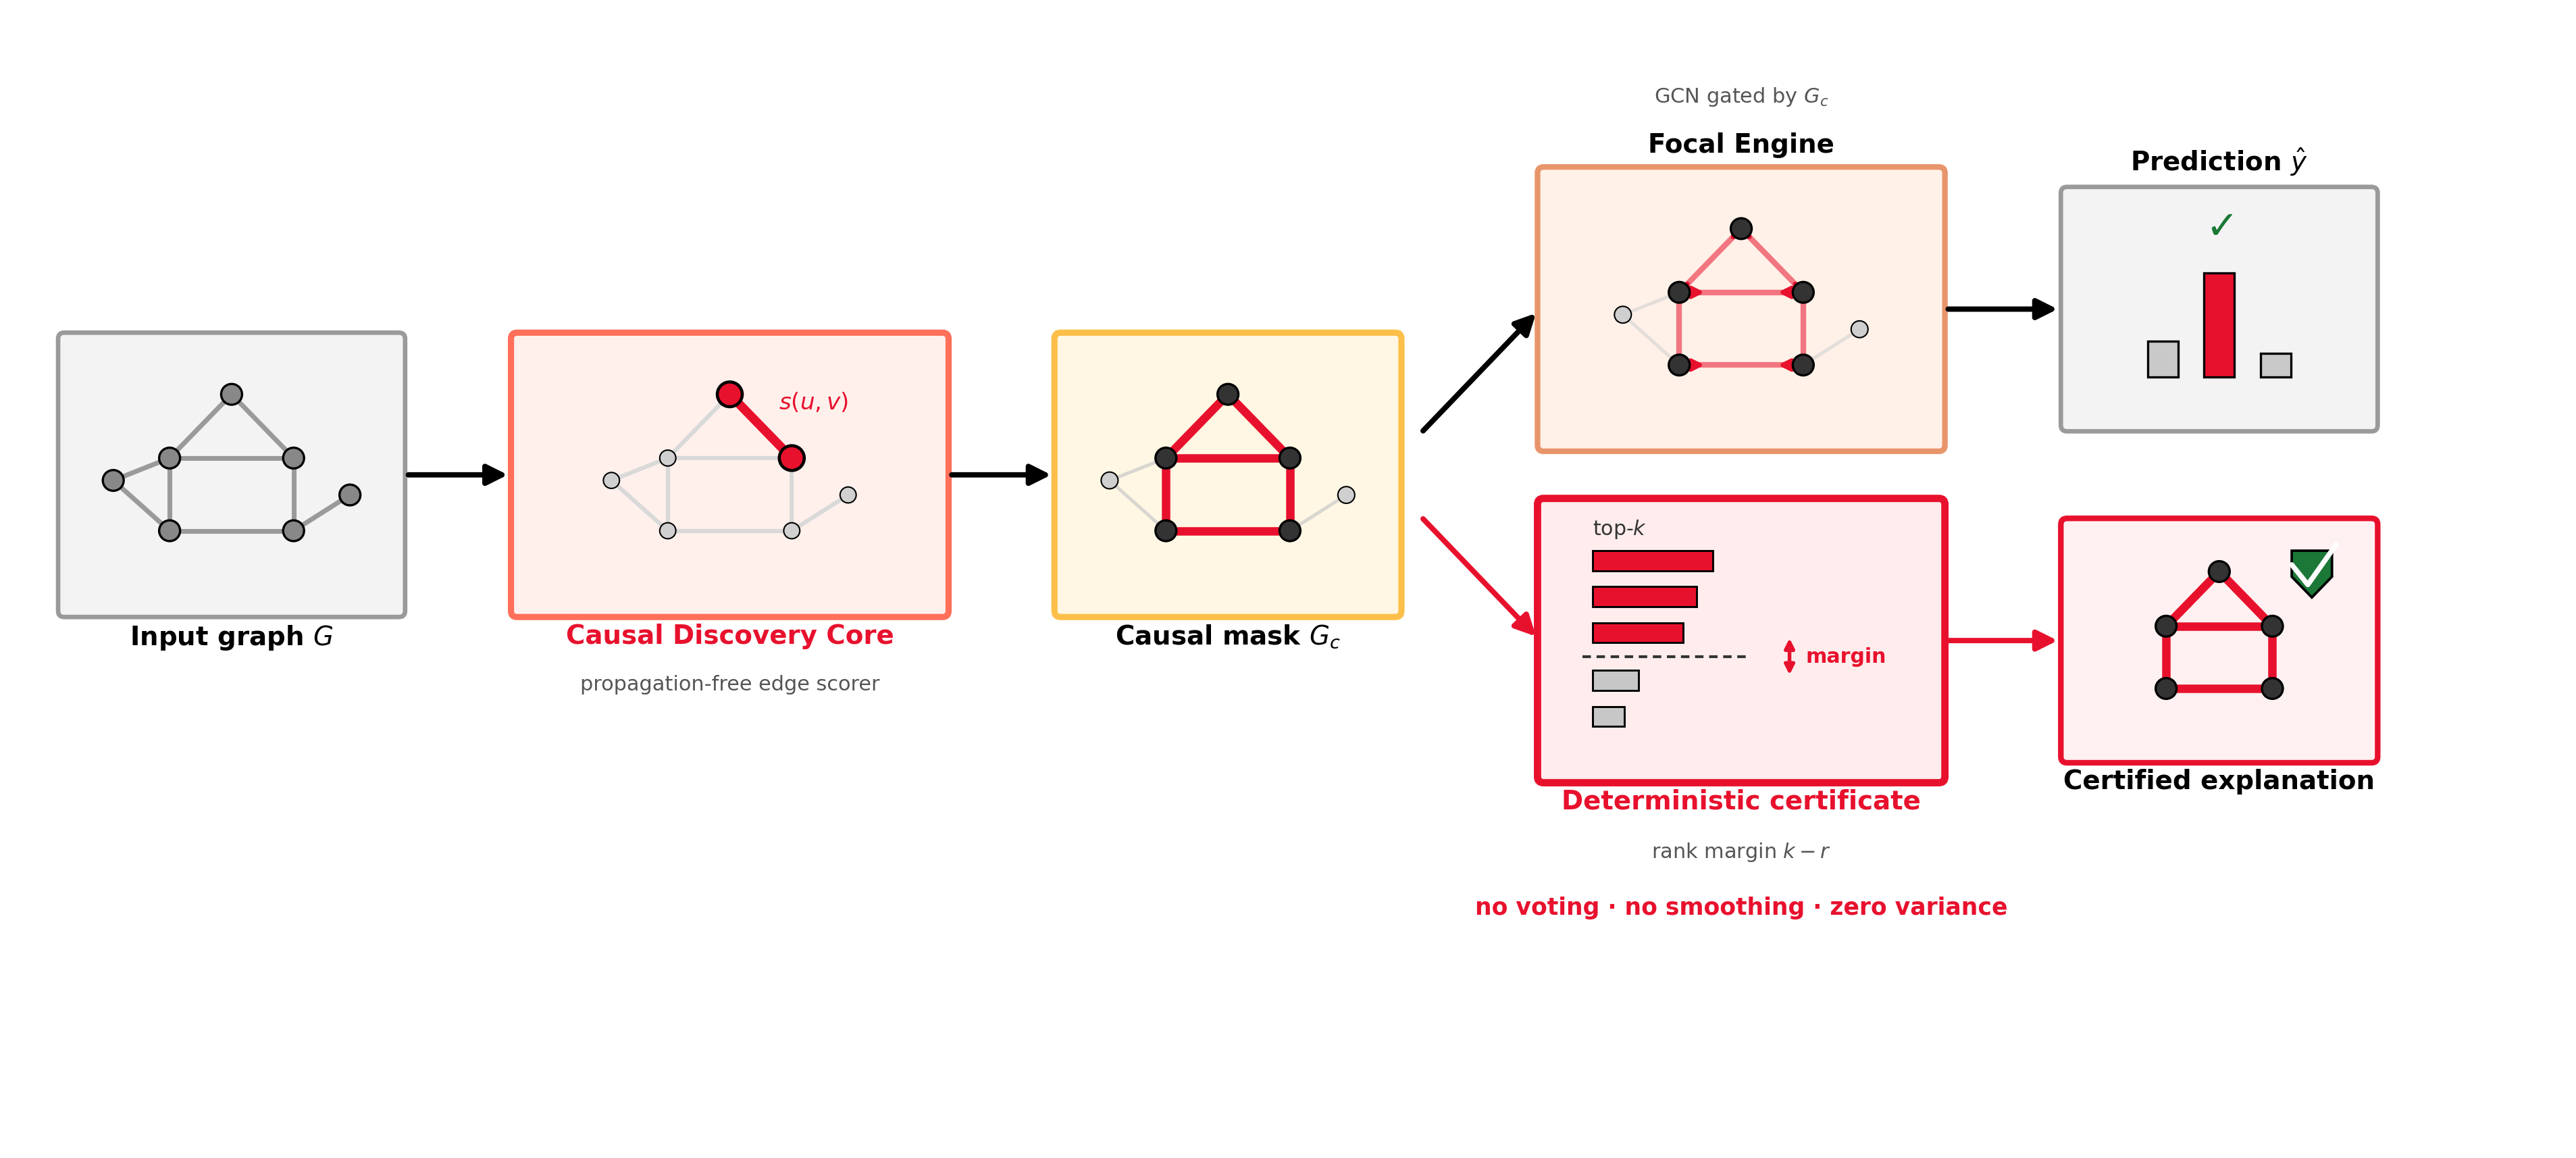
\includegraphics[width=\linewidth]{../../figures/F0_architecture.png}
  \caption{The \aeth{} pipeline: a propagation-free causal core scores each edge
  from its endpoints alone, producing a mask that gates prediction and feeds a
  \emph{deterministic} rank-margin certificate ($k-r$)---no voting, no
  smoothing.}
  \label{fig:arch}
\end{figure}

\begin{figure}[t]\centering
  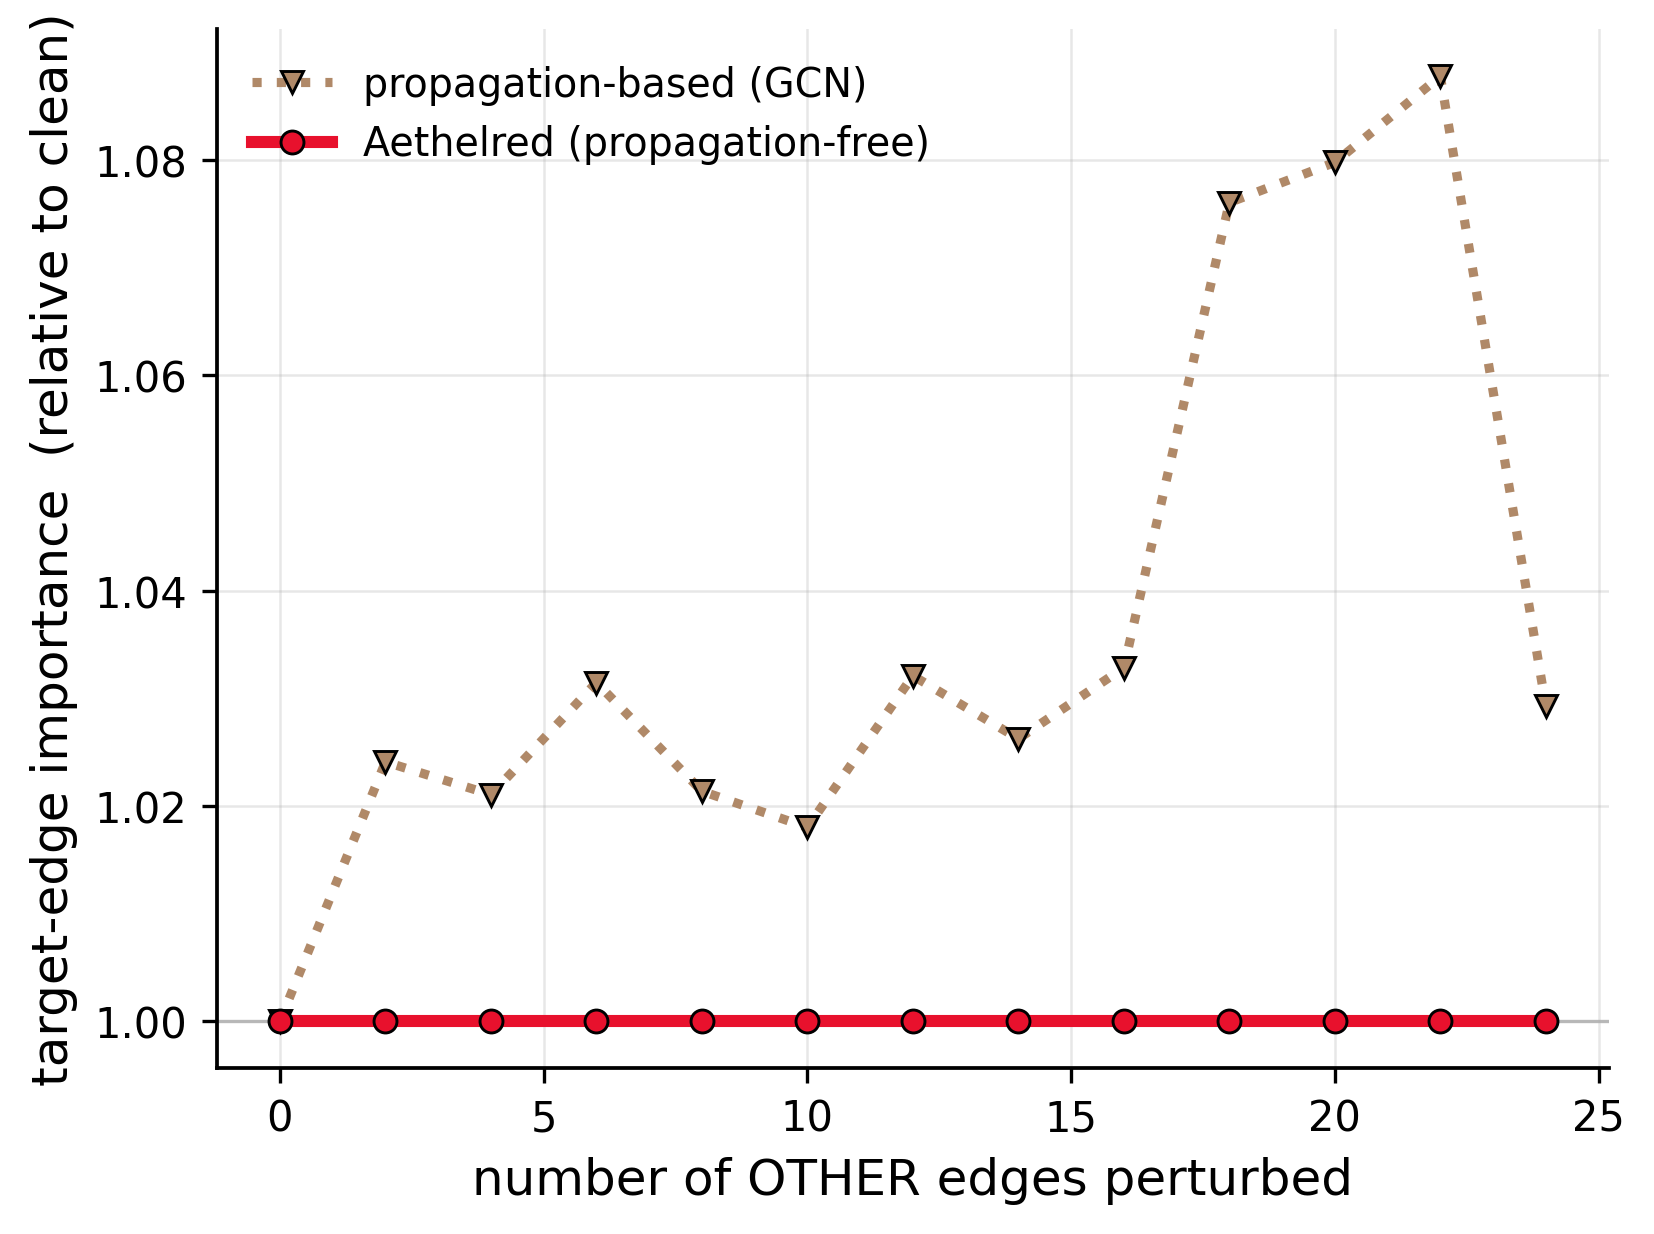
\includegraphics[width=0.82\linewidth]{../../figures/F10_edge_locality.png}
  \caption{Edge-locality. A target edge's importance vs.\ the number of
  \emph{other} edges perturbed: \aeth{}'s score is exactly invariant; a
  propagation-based (GCN) score drifts.}
  \label{fig:locality}
\end{figure}

\begin{figure}[t]\centering
  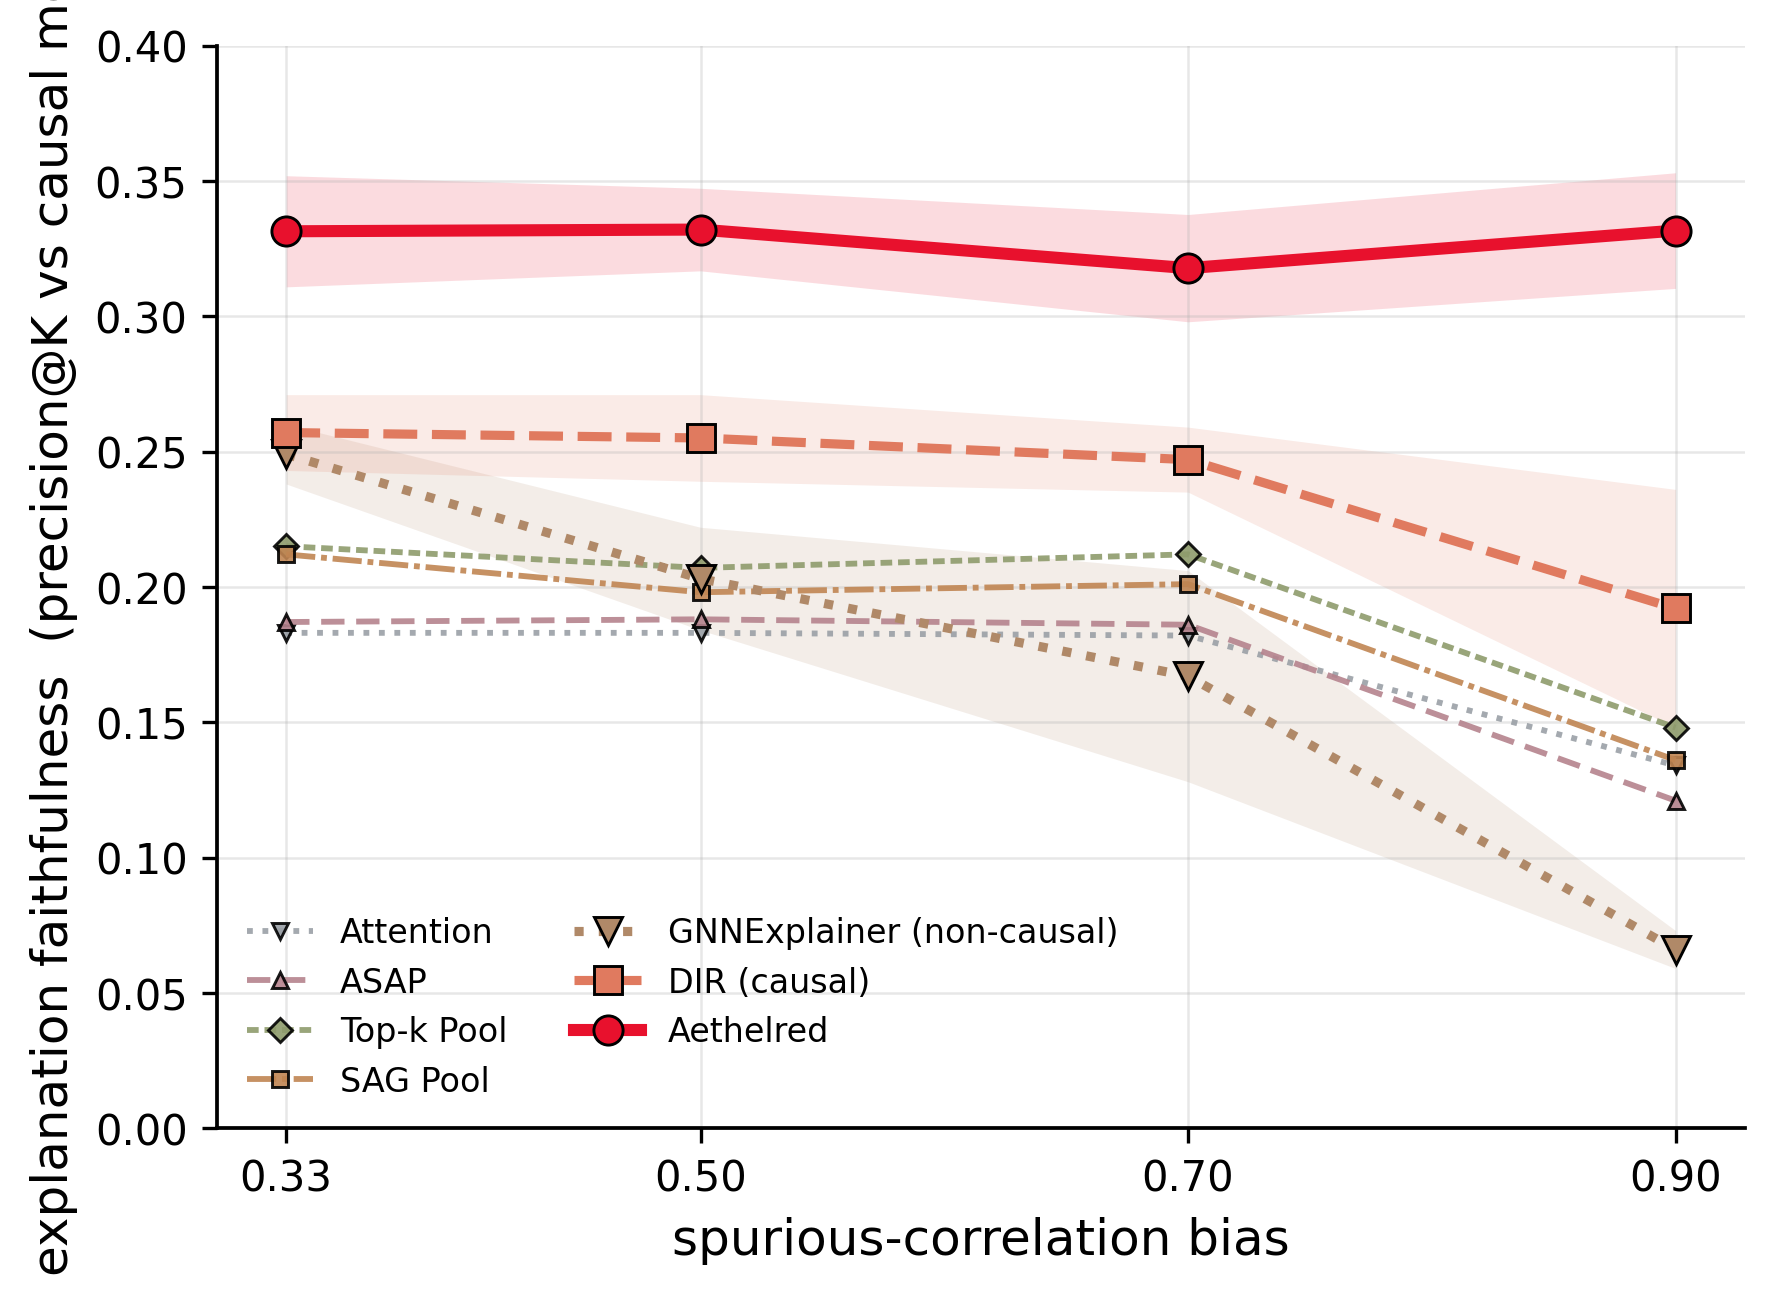
\includegraphics[width=0.9\linewidth]{../../figures/F9_spmotif_causal_vs_spurious.png}
  \caption{Faithfulness (precision@$K$ vs.\ the \emph{causal} motif) as spurious
  correlation strengthens on \textsc{SPMotif}. GNNExplainer and the pooling
  rationale baselines (Attention/ASAP/Top-k/SAG, DIR Table~2) collapse, DIR
  partly resists; \aeth{} is bias-invariant.}
  \label{fig:thesis}
\end{figure}

\begin{figure}[t]\centering
  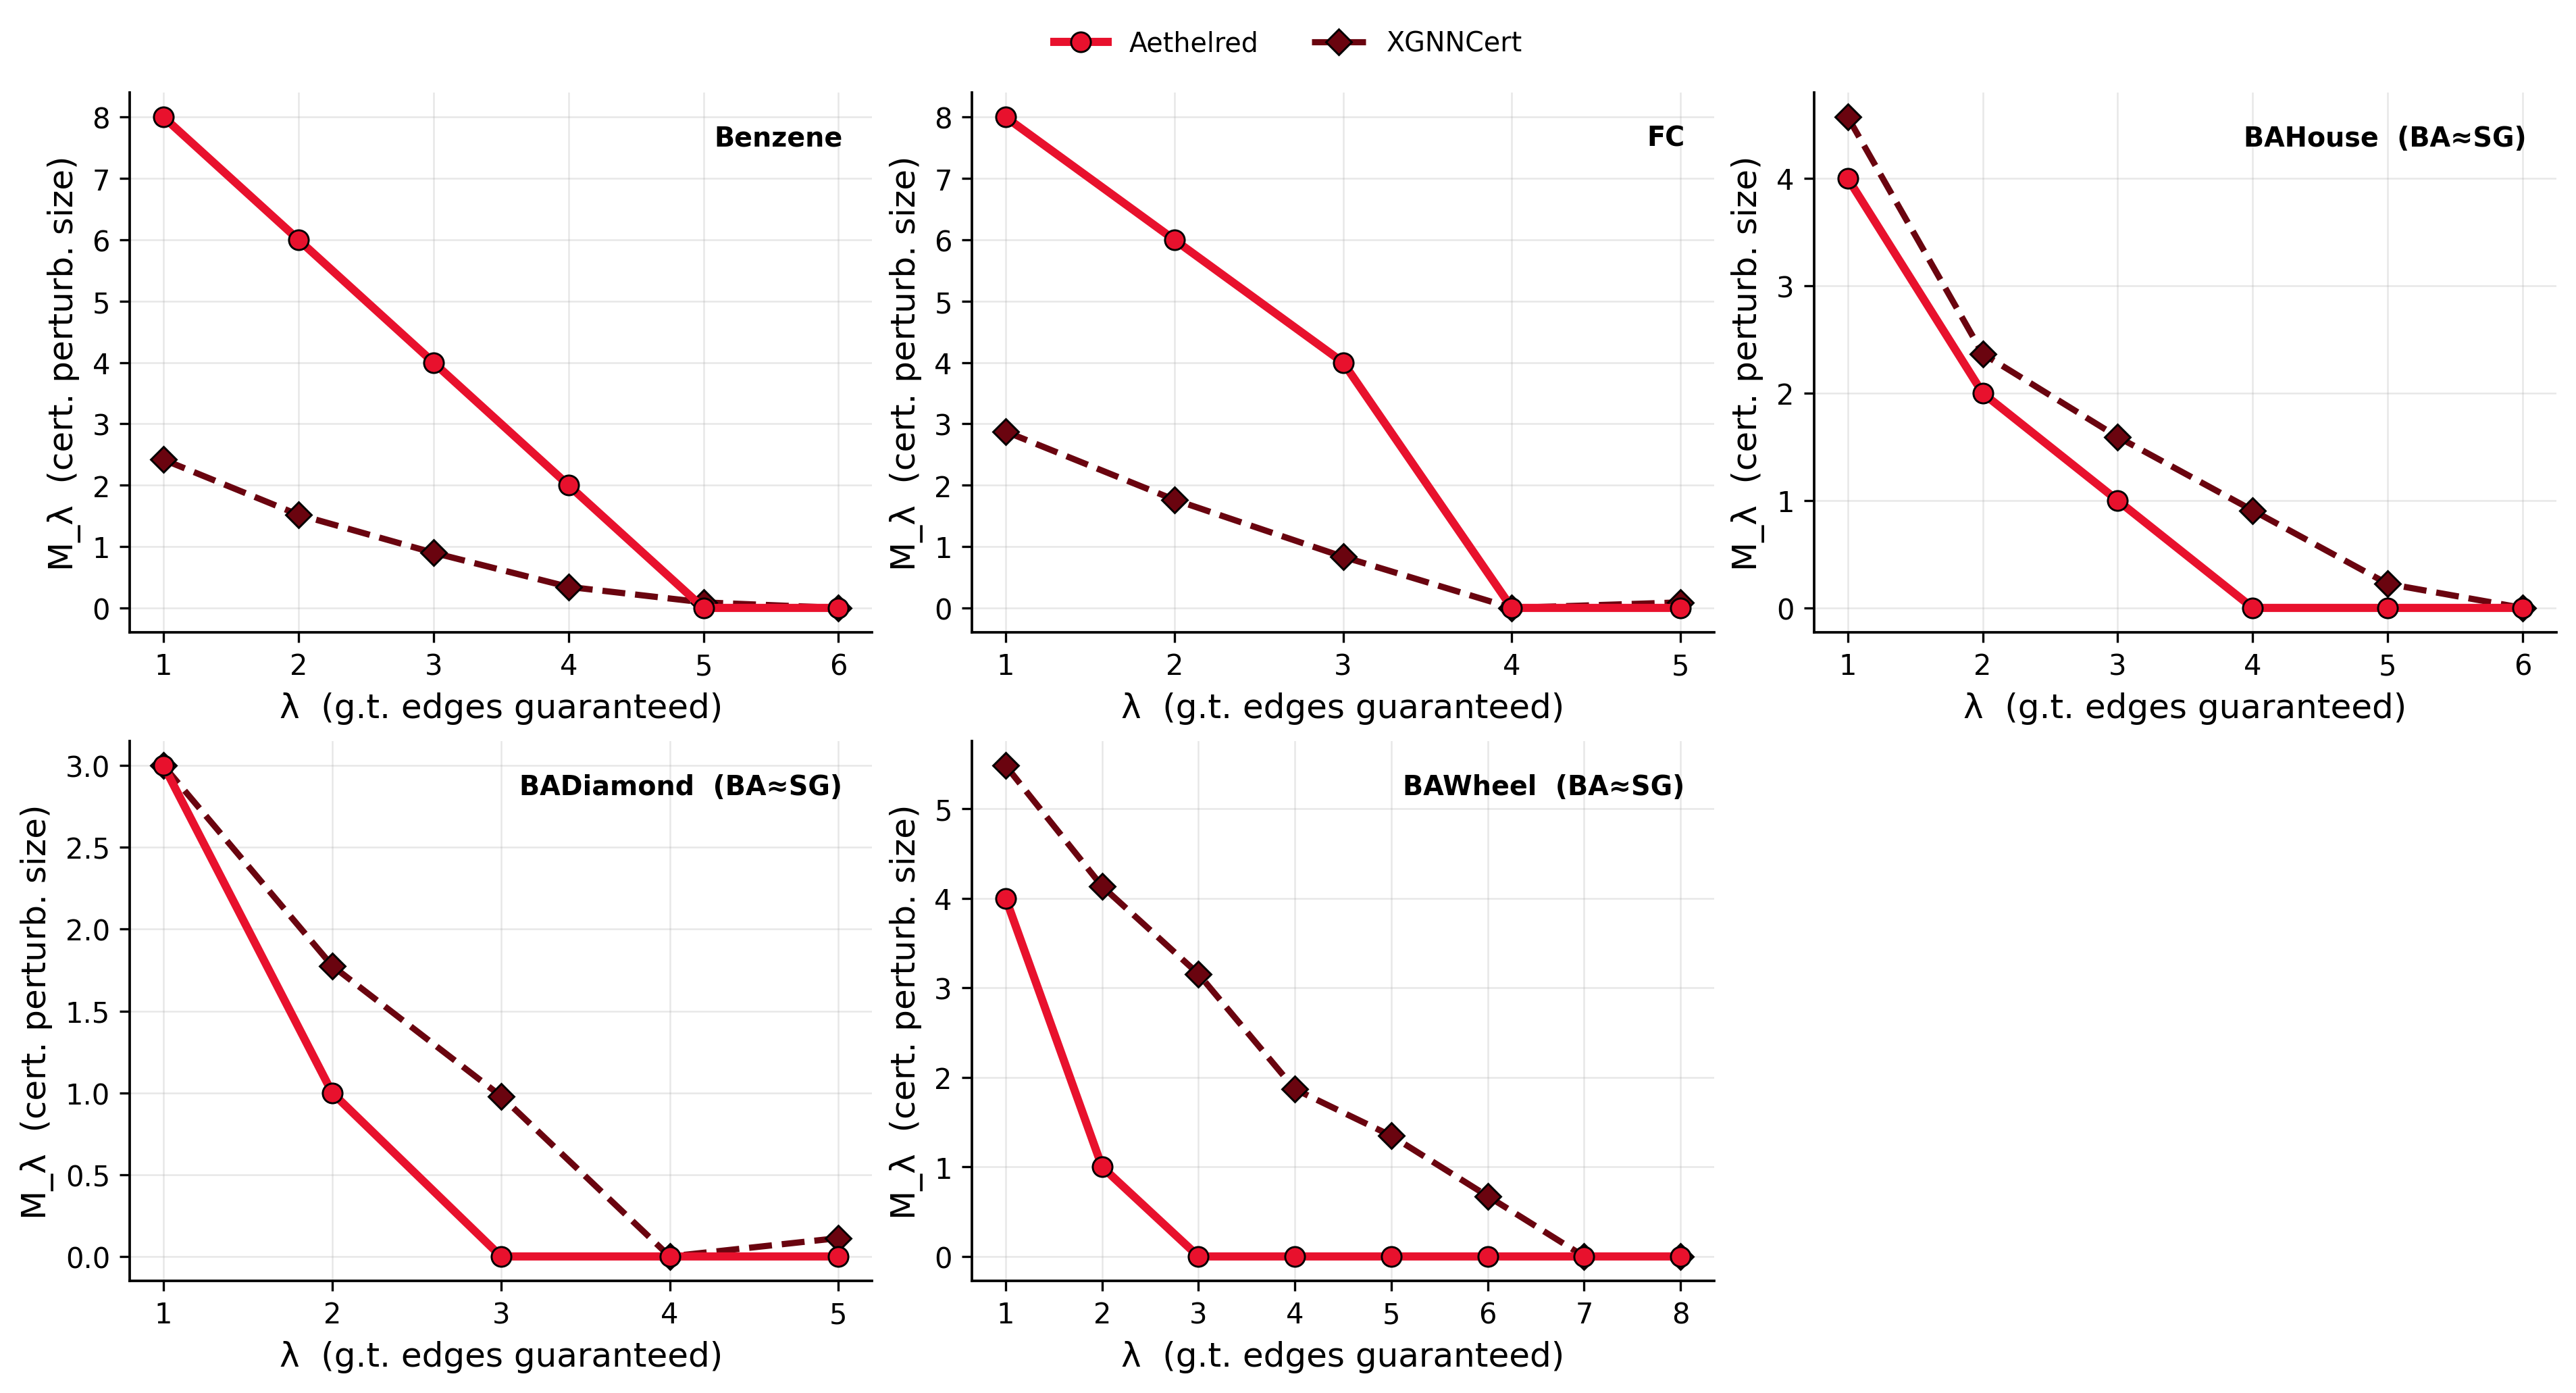
\includegraphics[width=\linewidth]{../../figures/F7_Mlambda_vs_lambda.png}
  \caption{Certified perturbation size $M_\lambda$ vs.\ guaranteed ground-truth
  edges $\lambda$ (\xgn{}'s own metric). \aeth{} vs.\ \xgn{}'s authoritative
  published default ($T{=}70$, PGExplainer).}
  \label{fig:mlambda}
\end{figure}

\begin{figure}[t]\centering
  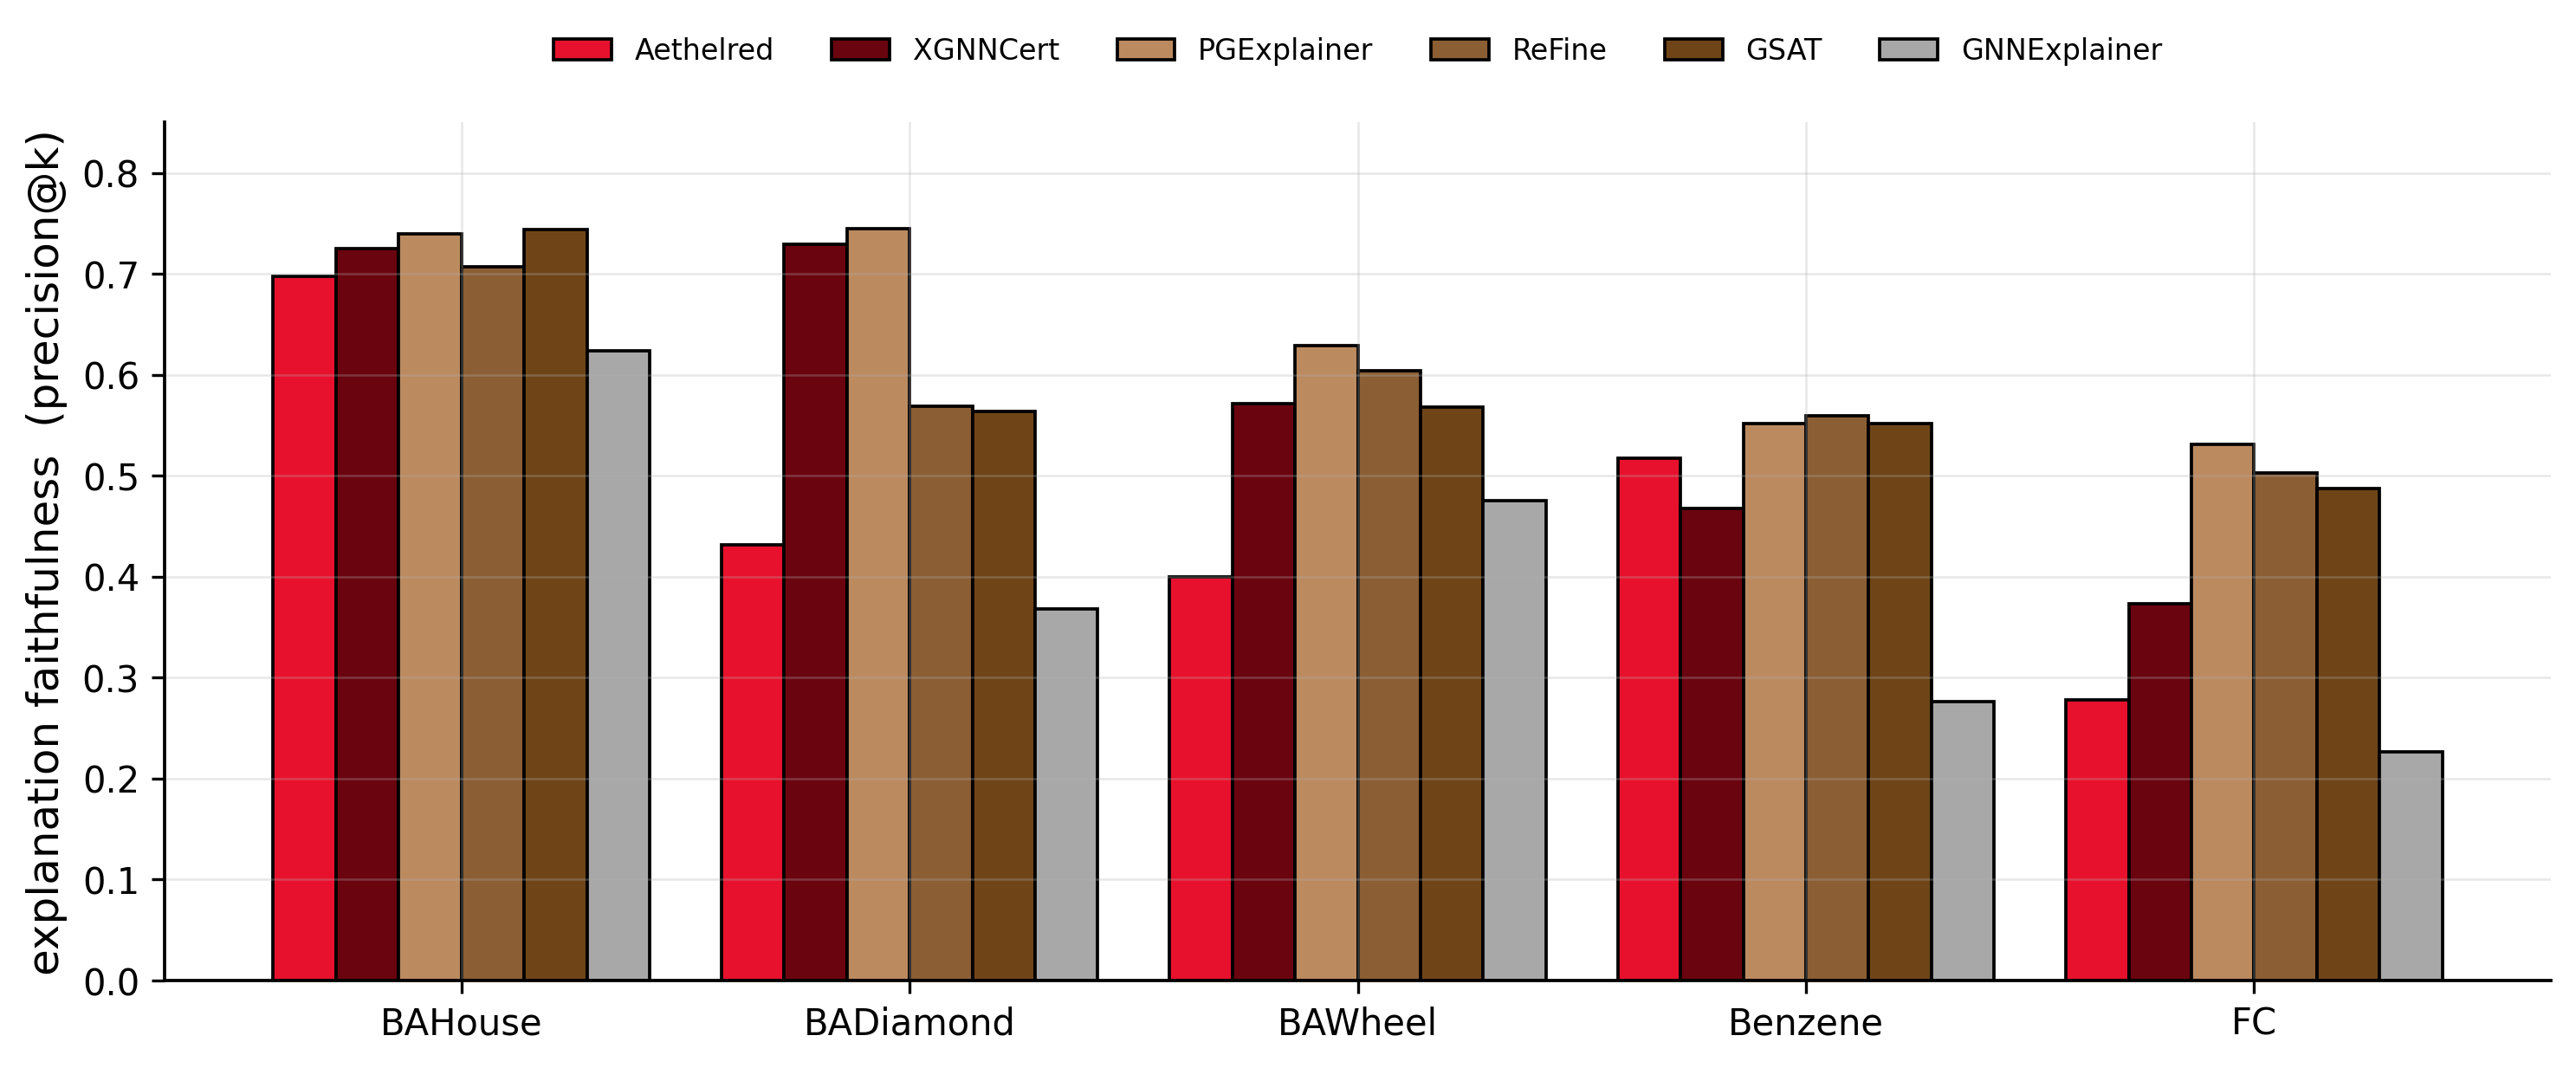
\includegraphics[width=\linewidth]{../../figures/F2c_unified_faithfulness.png}
  \caption{Clean explanation faithfulness: \aeth{} against all explanation
  baselines (\xgn{}, PGExplainer, ReFine, GSAT, GNNExplainer) on the five
  ground-truth-motif datasets.}
  \label{fig:unifaith}
\end{figure}

\begin{figure}[t]\centering
  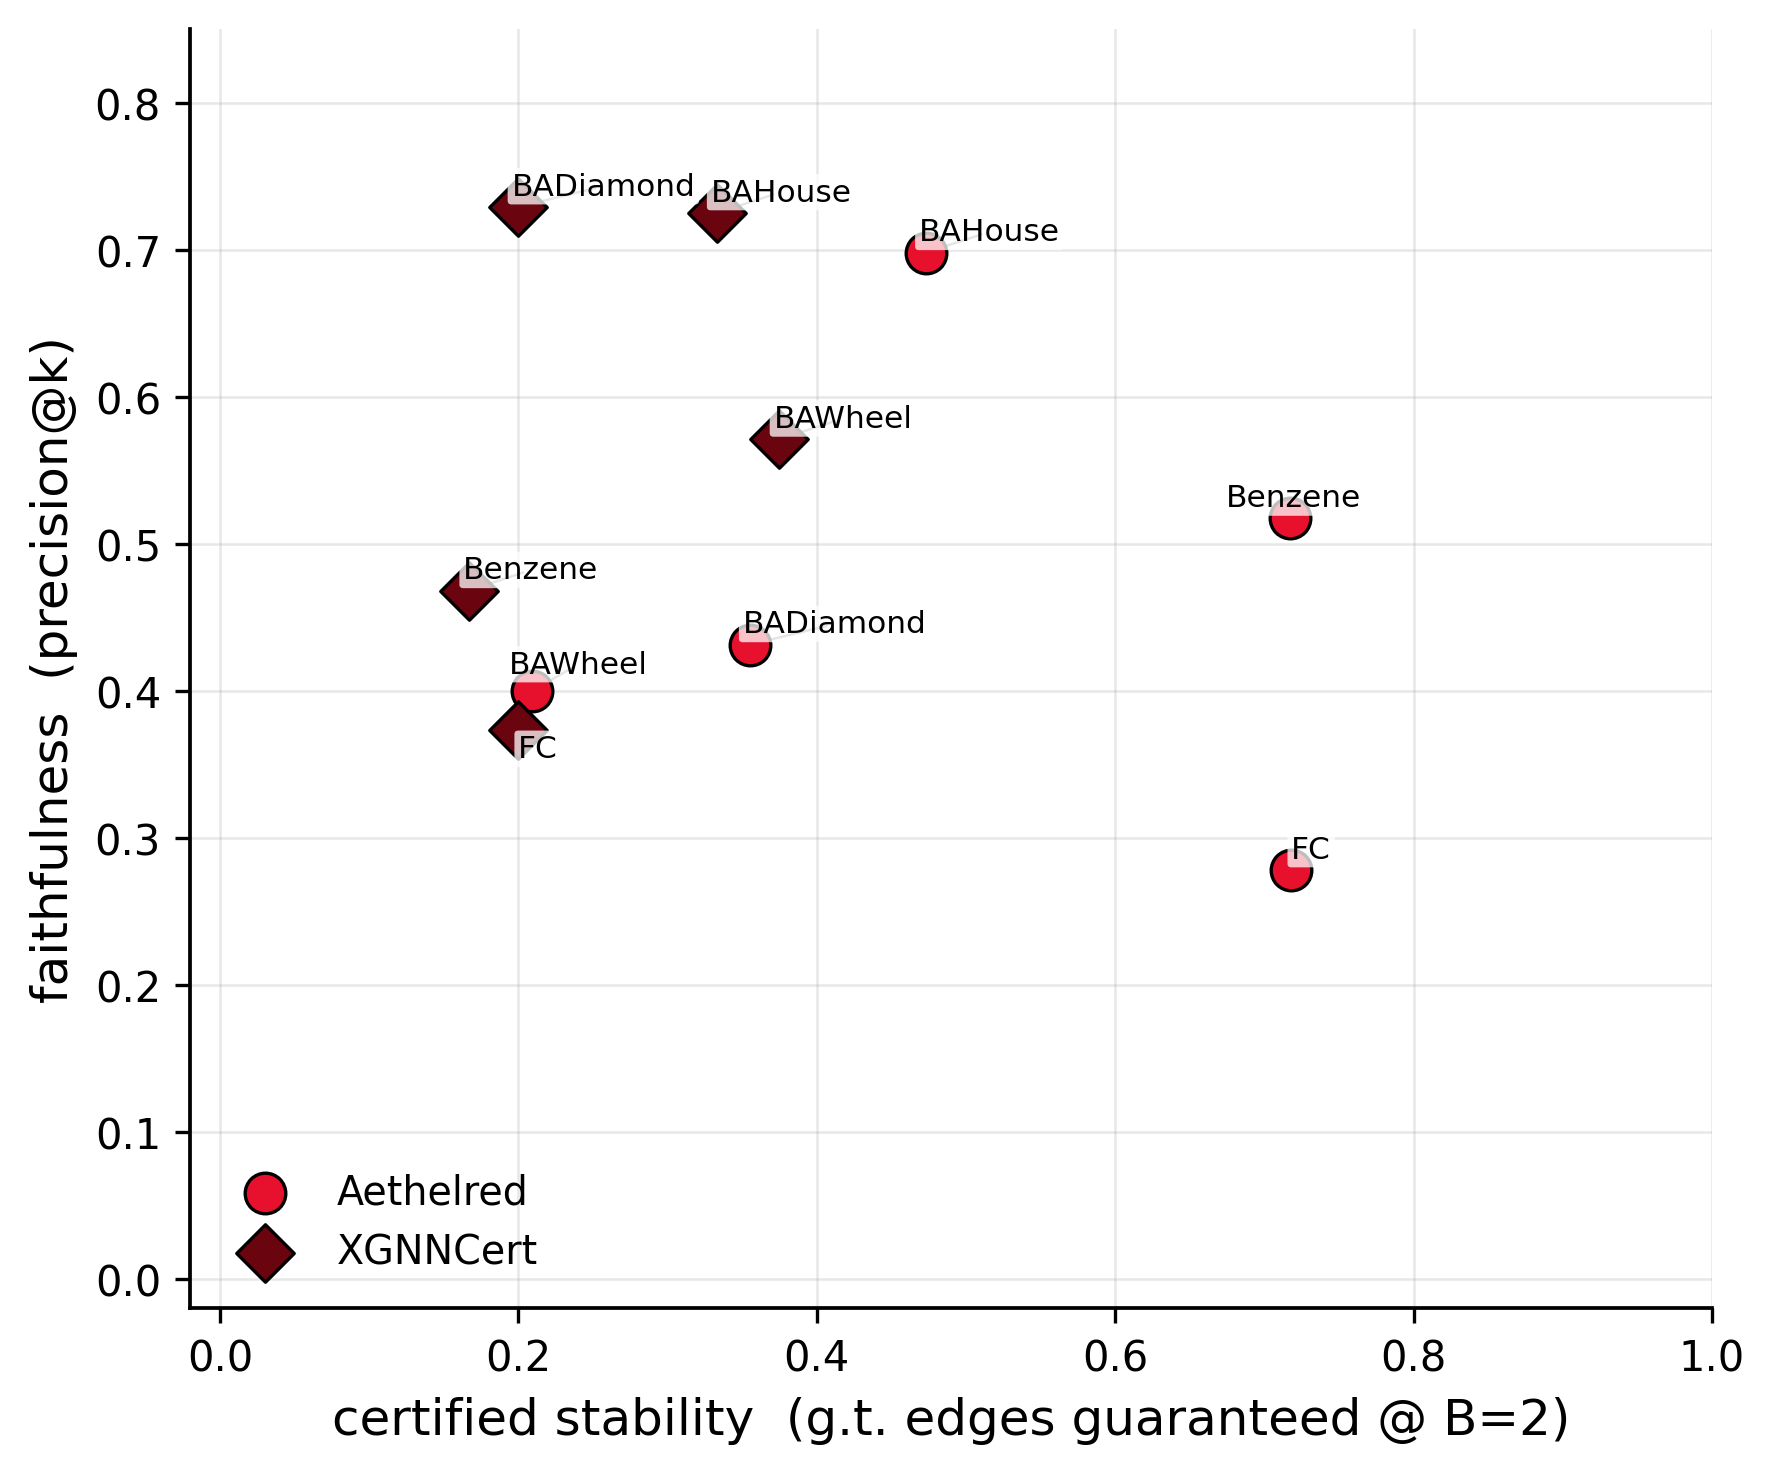
\includegraphics[width=0.85\linewidth]{../../figures/F3_faithfulness_stability_frontier.png}
  \caption{Faithfulness vs.\ certified stability (ground-truth edges guaranteed at
  $B{=}2$). Top-right is best; \xgn{} from published values.}
  \label{fig:frontier}
\end{figure}

\begin{figure}[t]\centering
  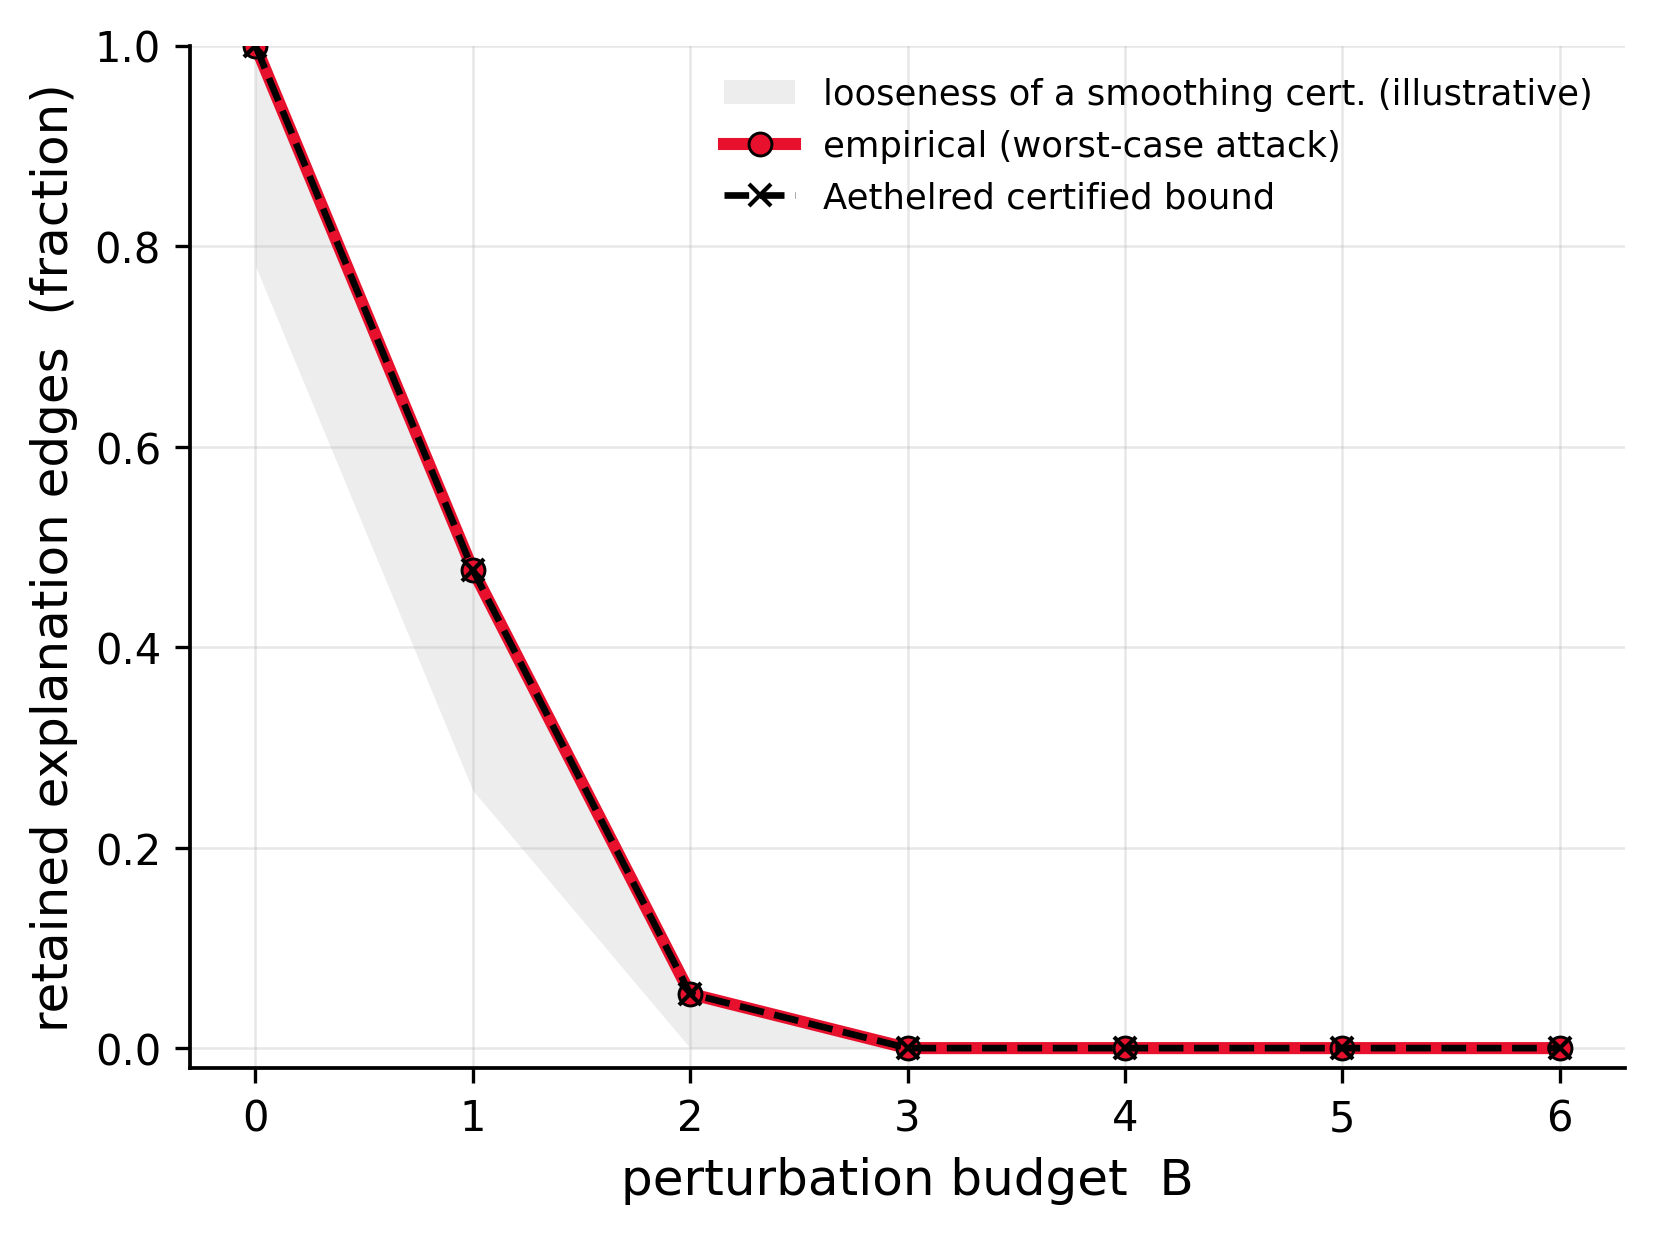
\includegraphics[width=0.82\linewidth]{../../figures/F11_certificate_tightness.png}
  \caption{Tightness: \aeth{}'s certified bound coincides with the empirical
  worst-case (gap $=0$); the grey band marks a smoothing certificate's looseness.}
  \label{fig:tight}
\end{figure}

\begin{figure}[t]\centering
  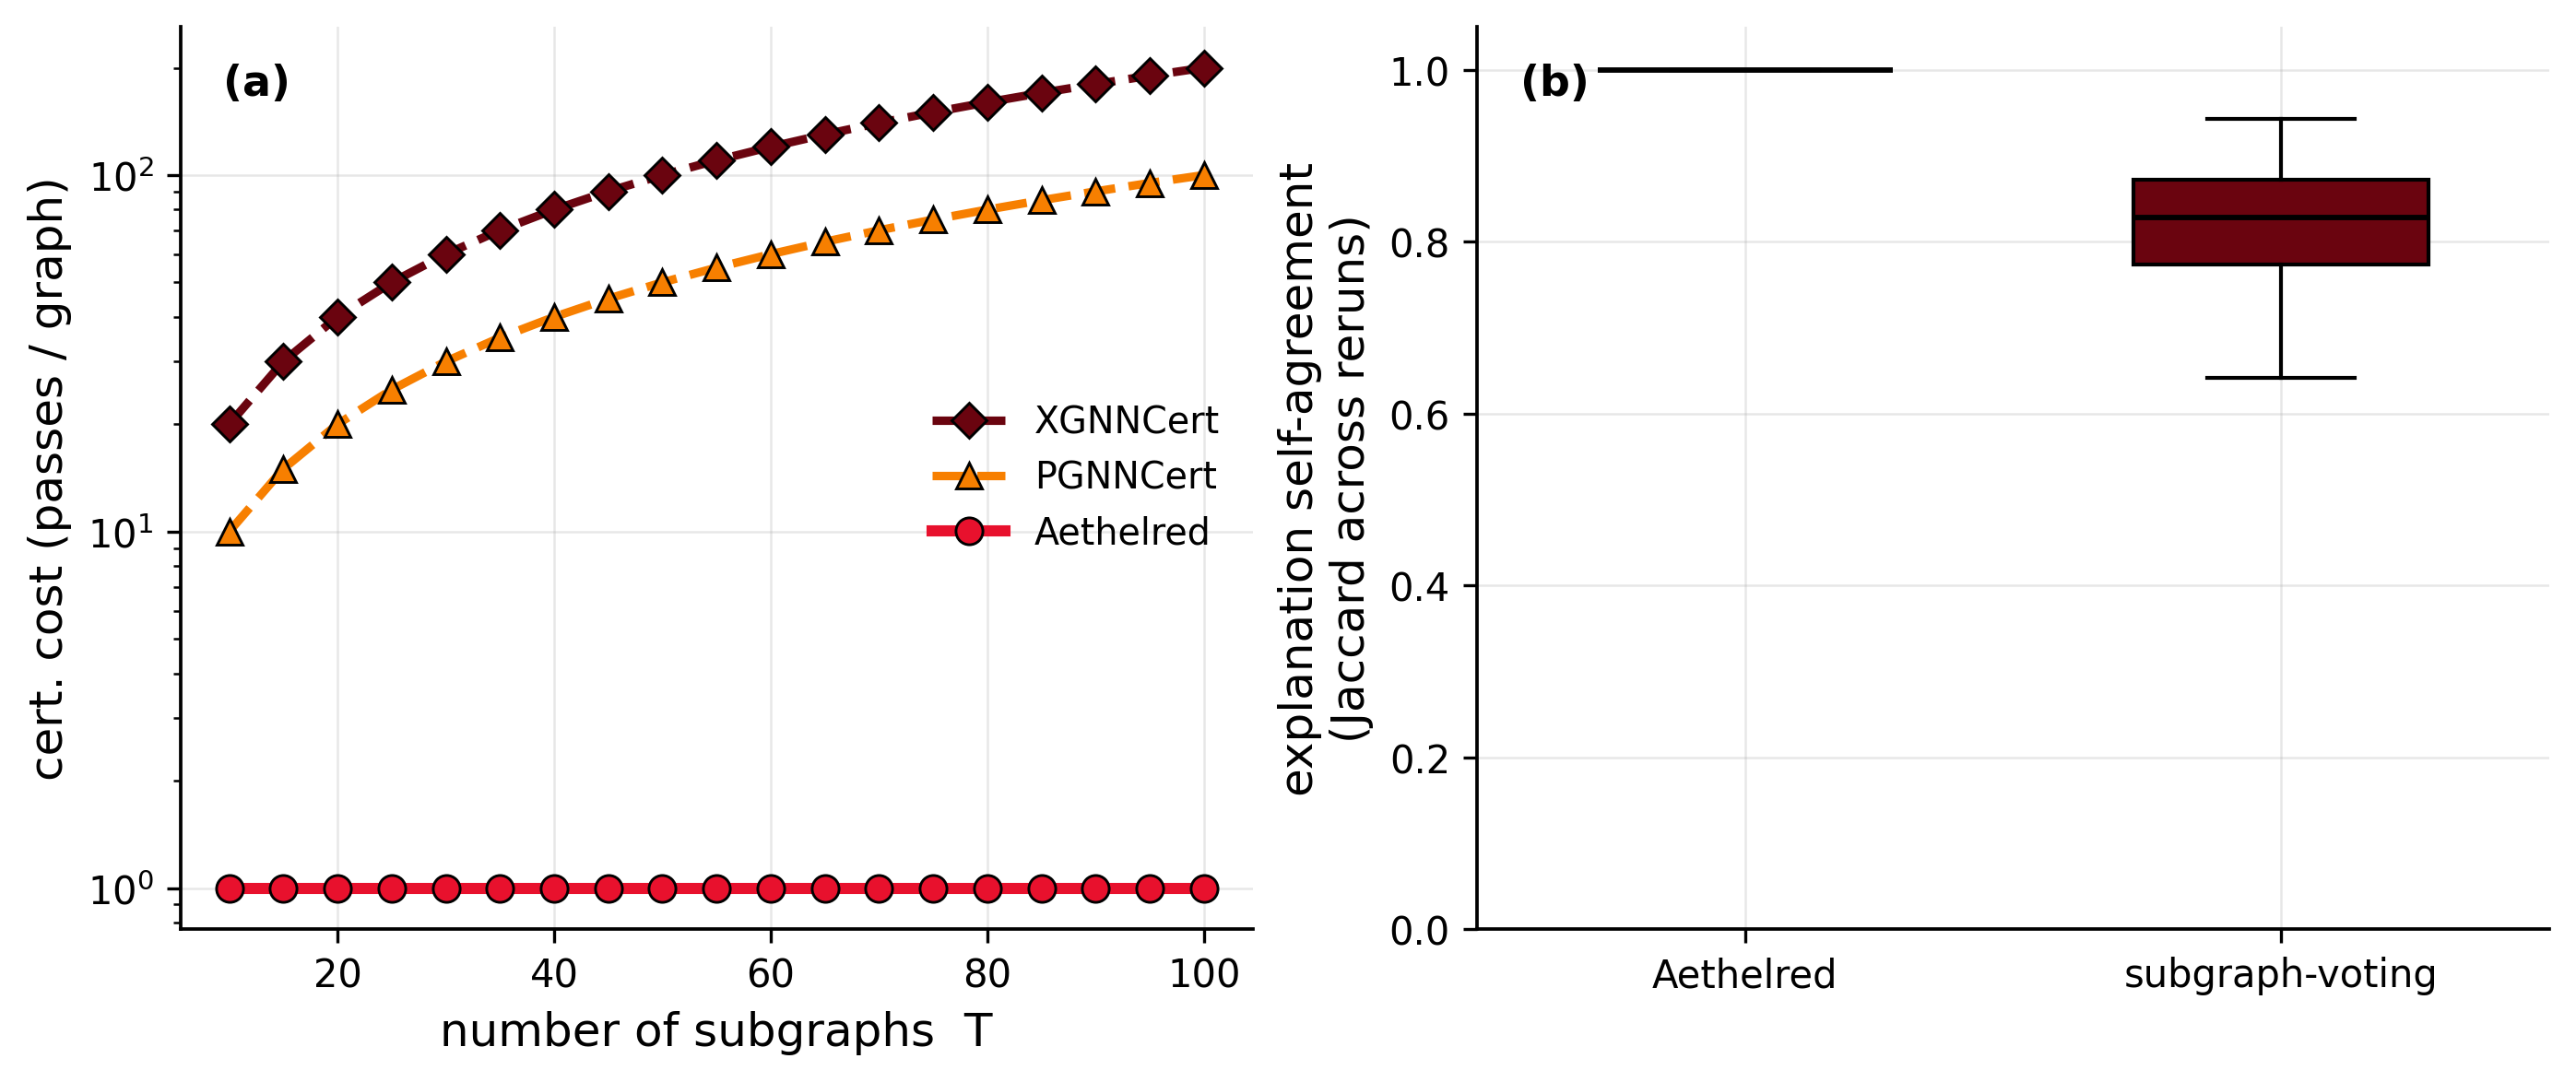
\includegraphics[width=\linewidth]{../../figures/F56_efficiency_determinism.png}
  \caption{(a) Certification cost vs.\ \#sub-graphs $T$ (log scale).
  (b) Explanation self-agreement across reruns.}
  \label{fig:eff}
\end{figure}

\begin{figure}[t]\centering
  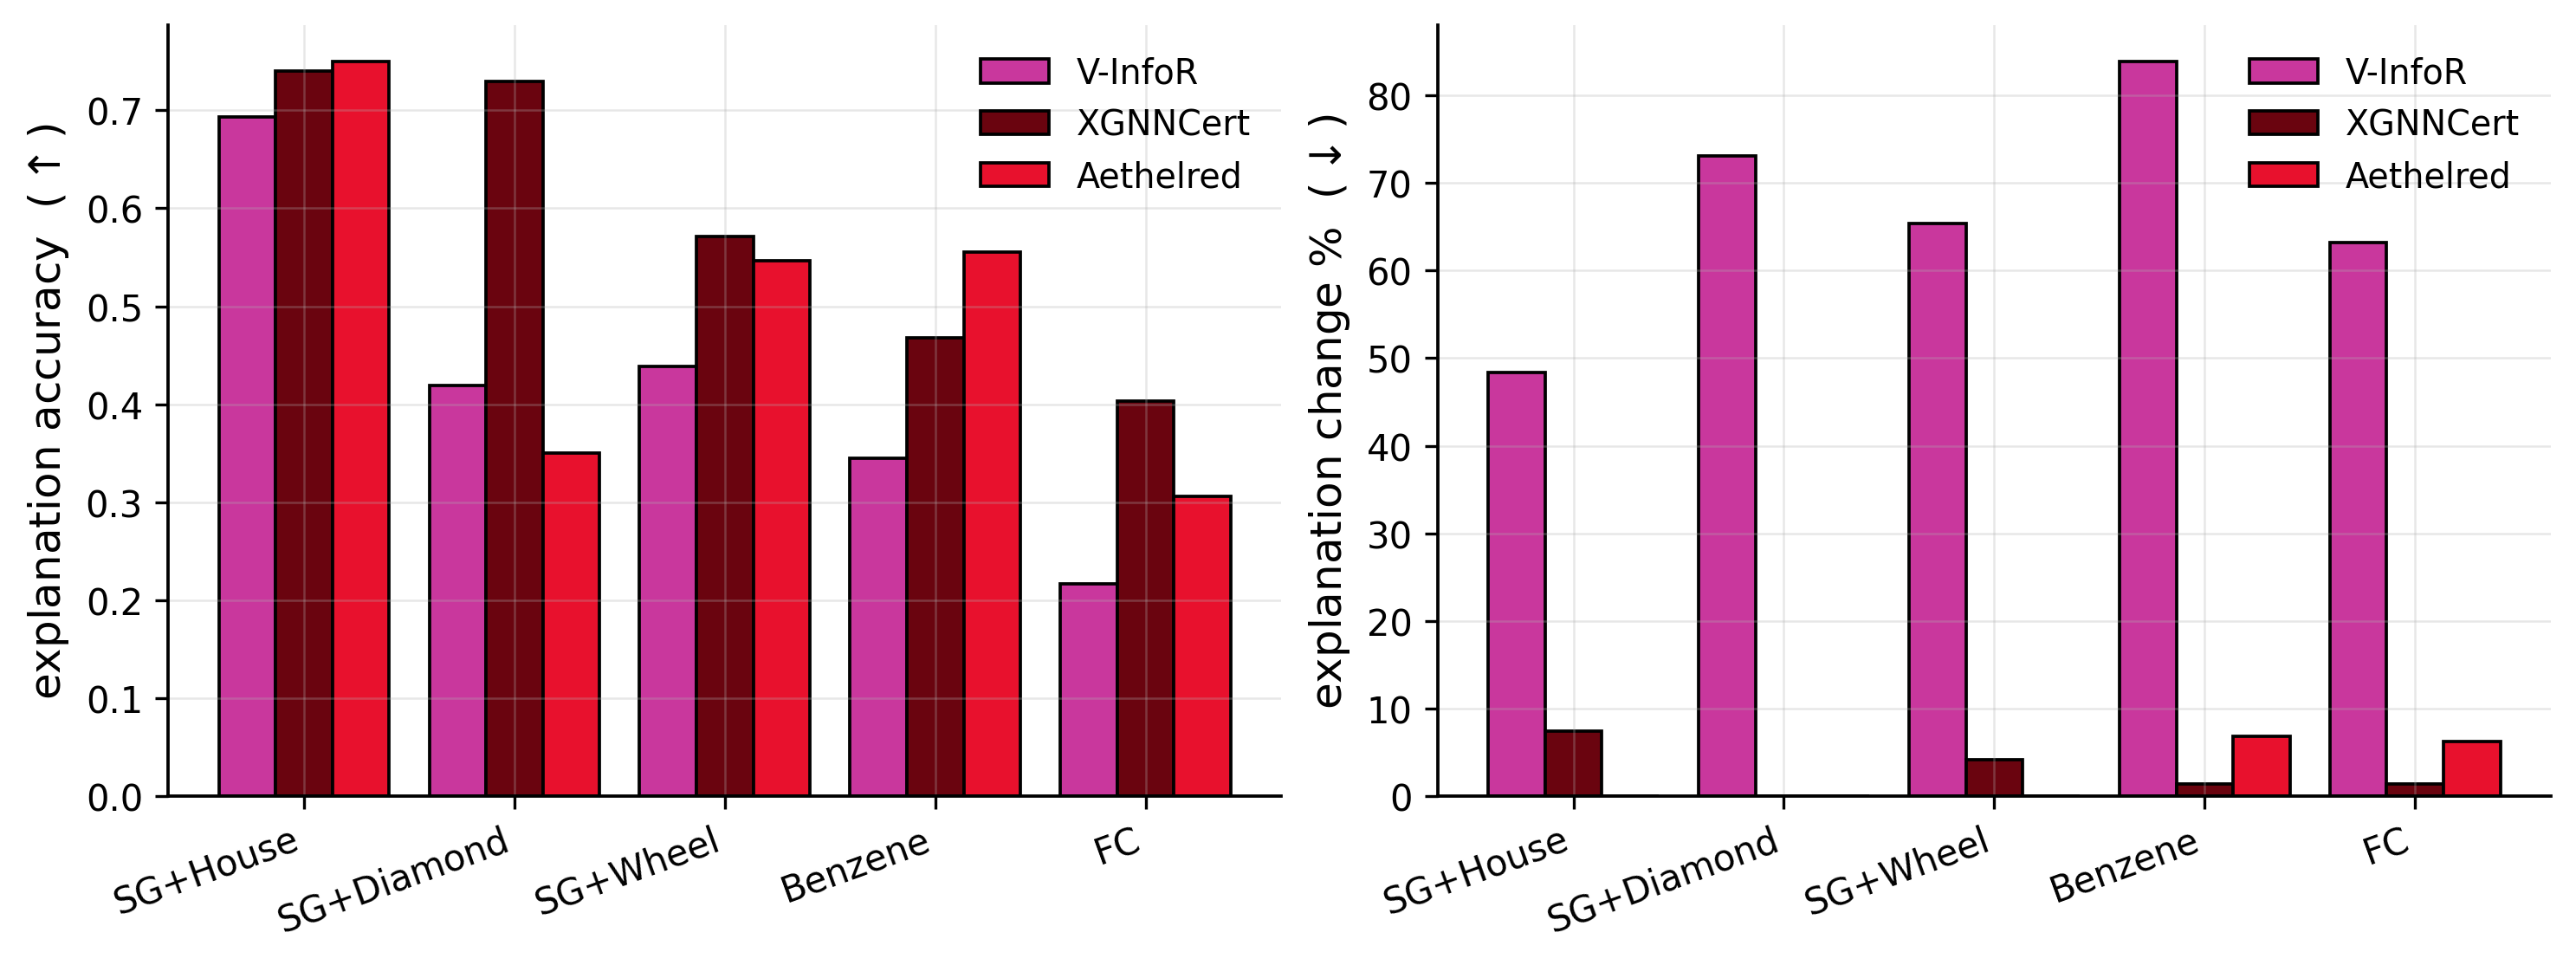
\includegraphics[width=\linewidth]{../../figures/F2b_explanation_robustness_vs_VInfoR.png}
  \caption{Explanation robustness under a $2$-edge attack: faithfulness
  ($\uparrow$) and drift ($\downarrow$) for \aeth{}, \xgn{}, and
  \textcolor{vinfomag}{V-InfoR}.}
  \label{fig:attack}
\end{figure}

\begin{figure}[t]\centering
  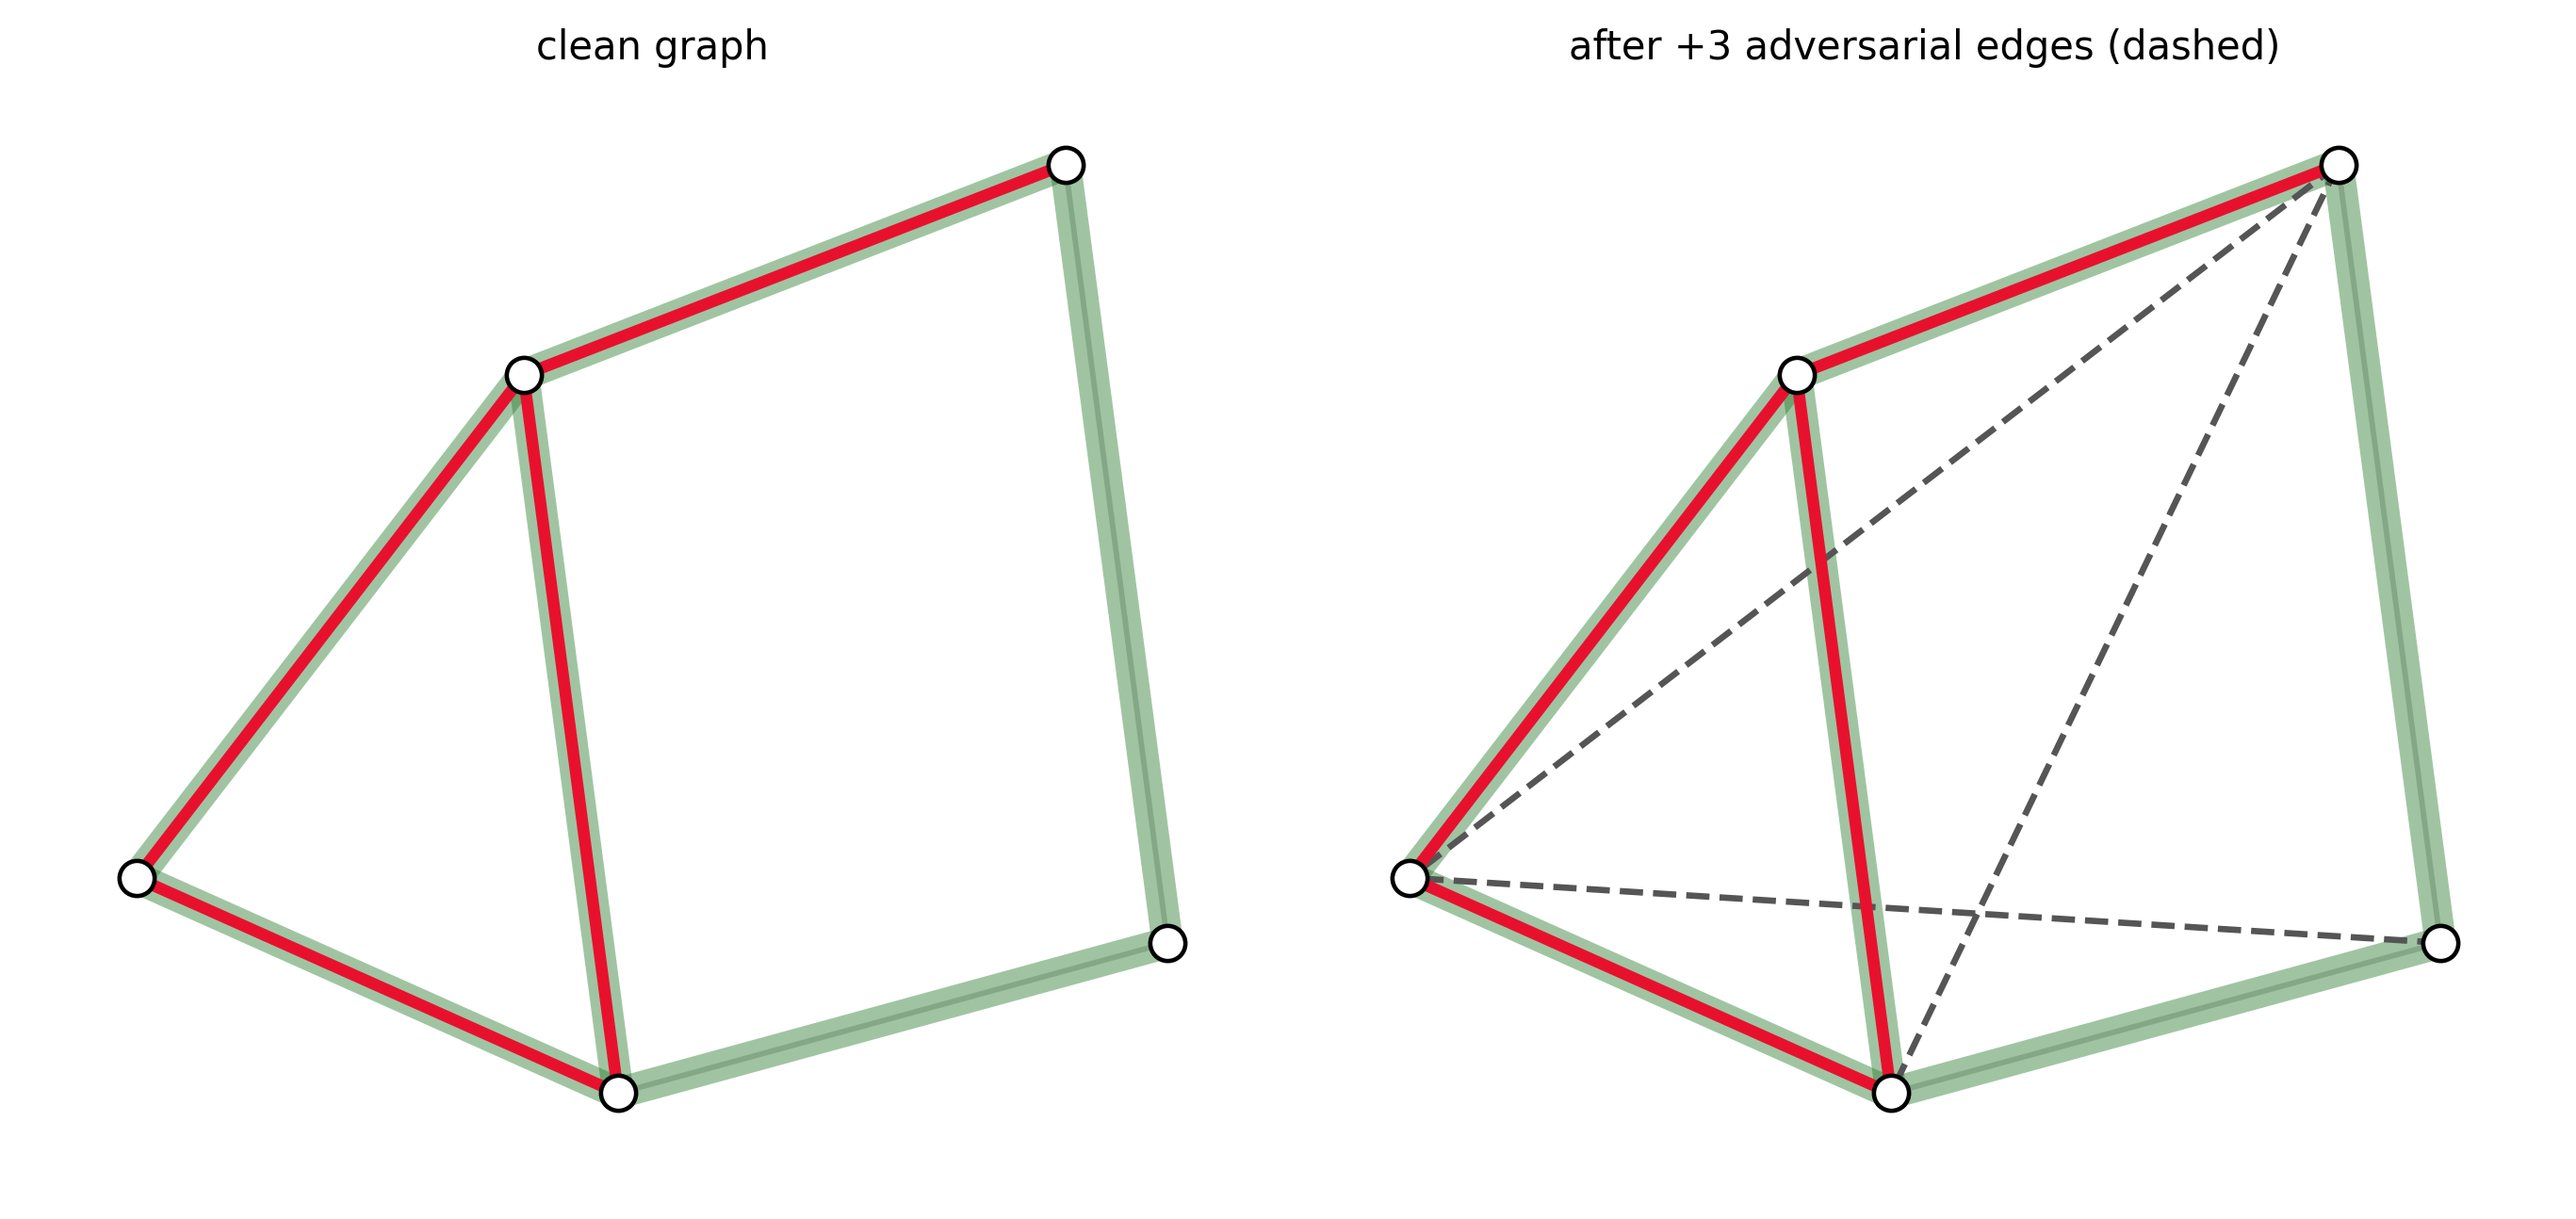
\includegraphics[width=\linewidth]{../../figures/F4_qualitative_explanation.png}
  \caption{\aeth{}'s certified explanation (red) on the ground-truth motif
  (green), before/after $3$ adversarial edges (dashed): the certified subset is
  unchanged.}
  \label{fig:qual}
\end{figure}

\begin{figure}[t]\centering
  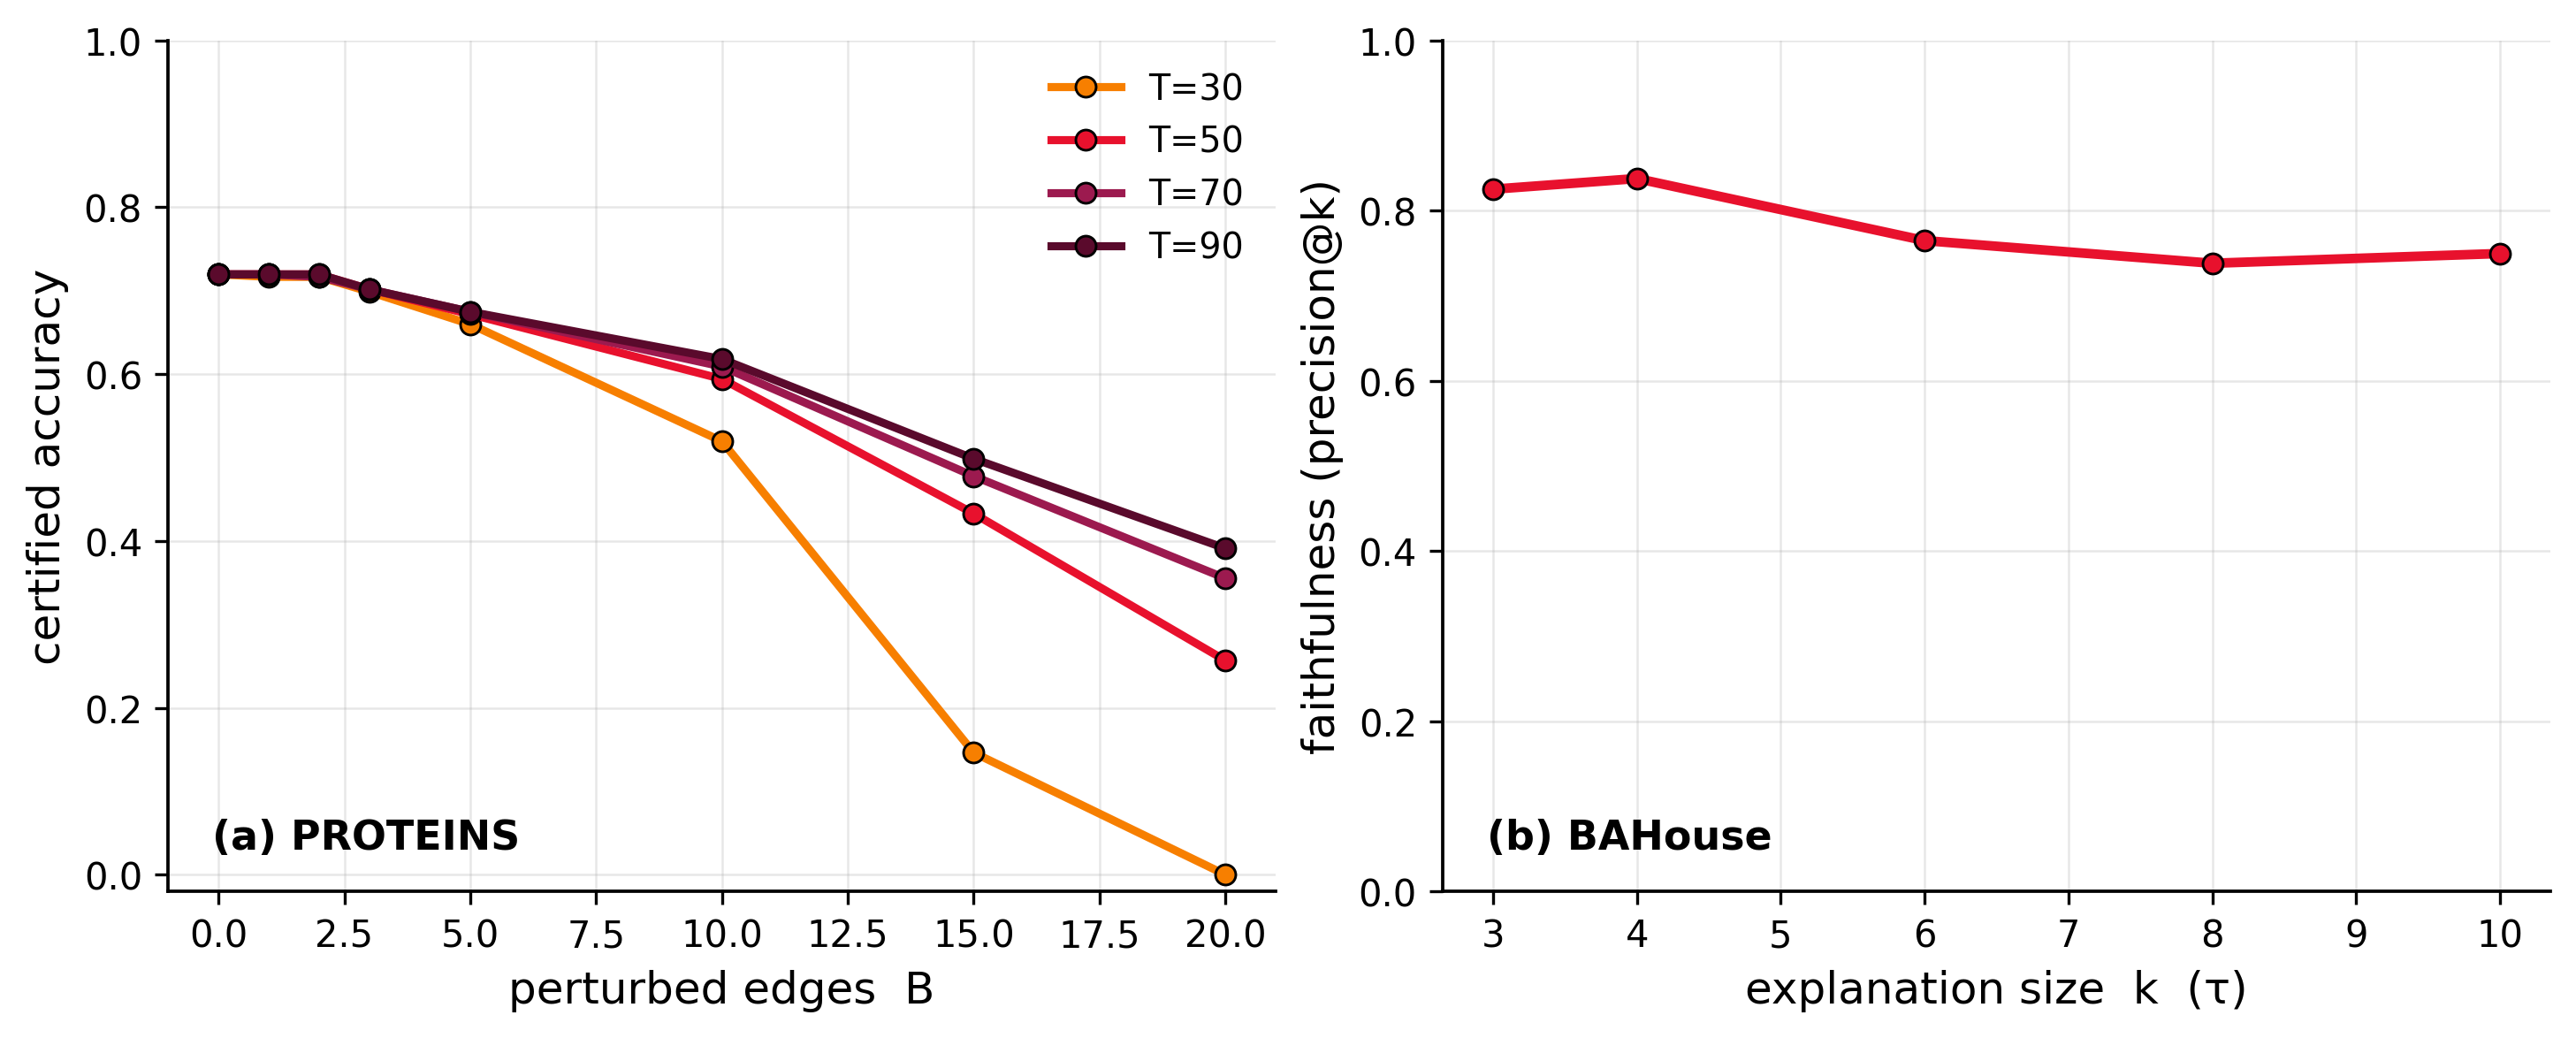
\includegraphics[width=\linewidth]{../../figures/F8_sensitivity.png}
  \caption{(a) Certified accuracy vs.\ budget for $T\!\in\!\{30,50,70,90\}$.
  (b) Faithfulness vs.\ explanation size $k$.}
  \label{fig:sens}
\end{figure}

\begin{figure}[t]\centering
  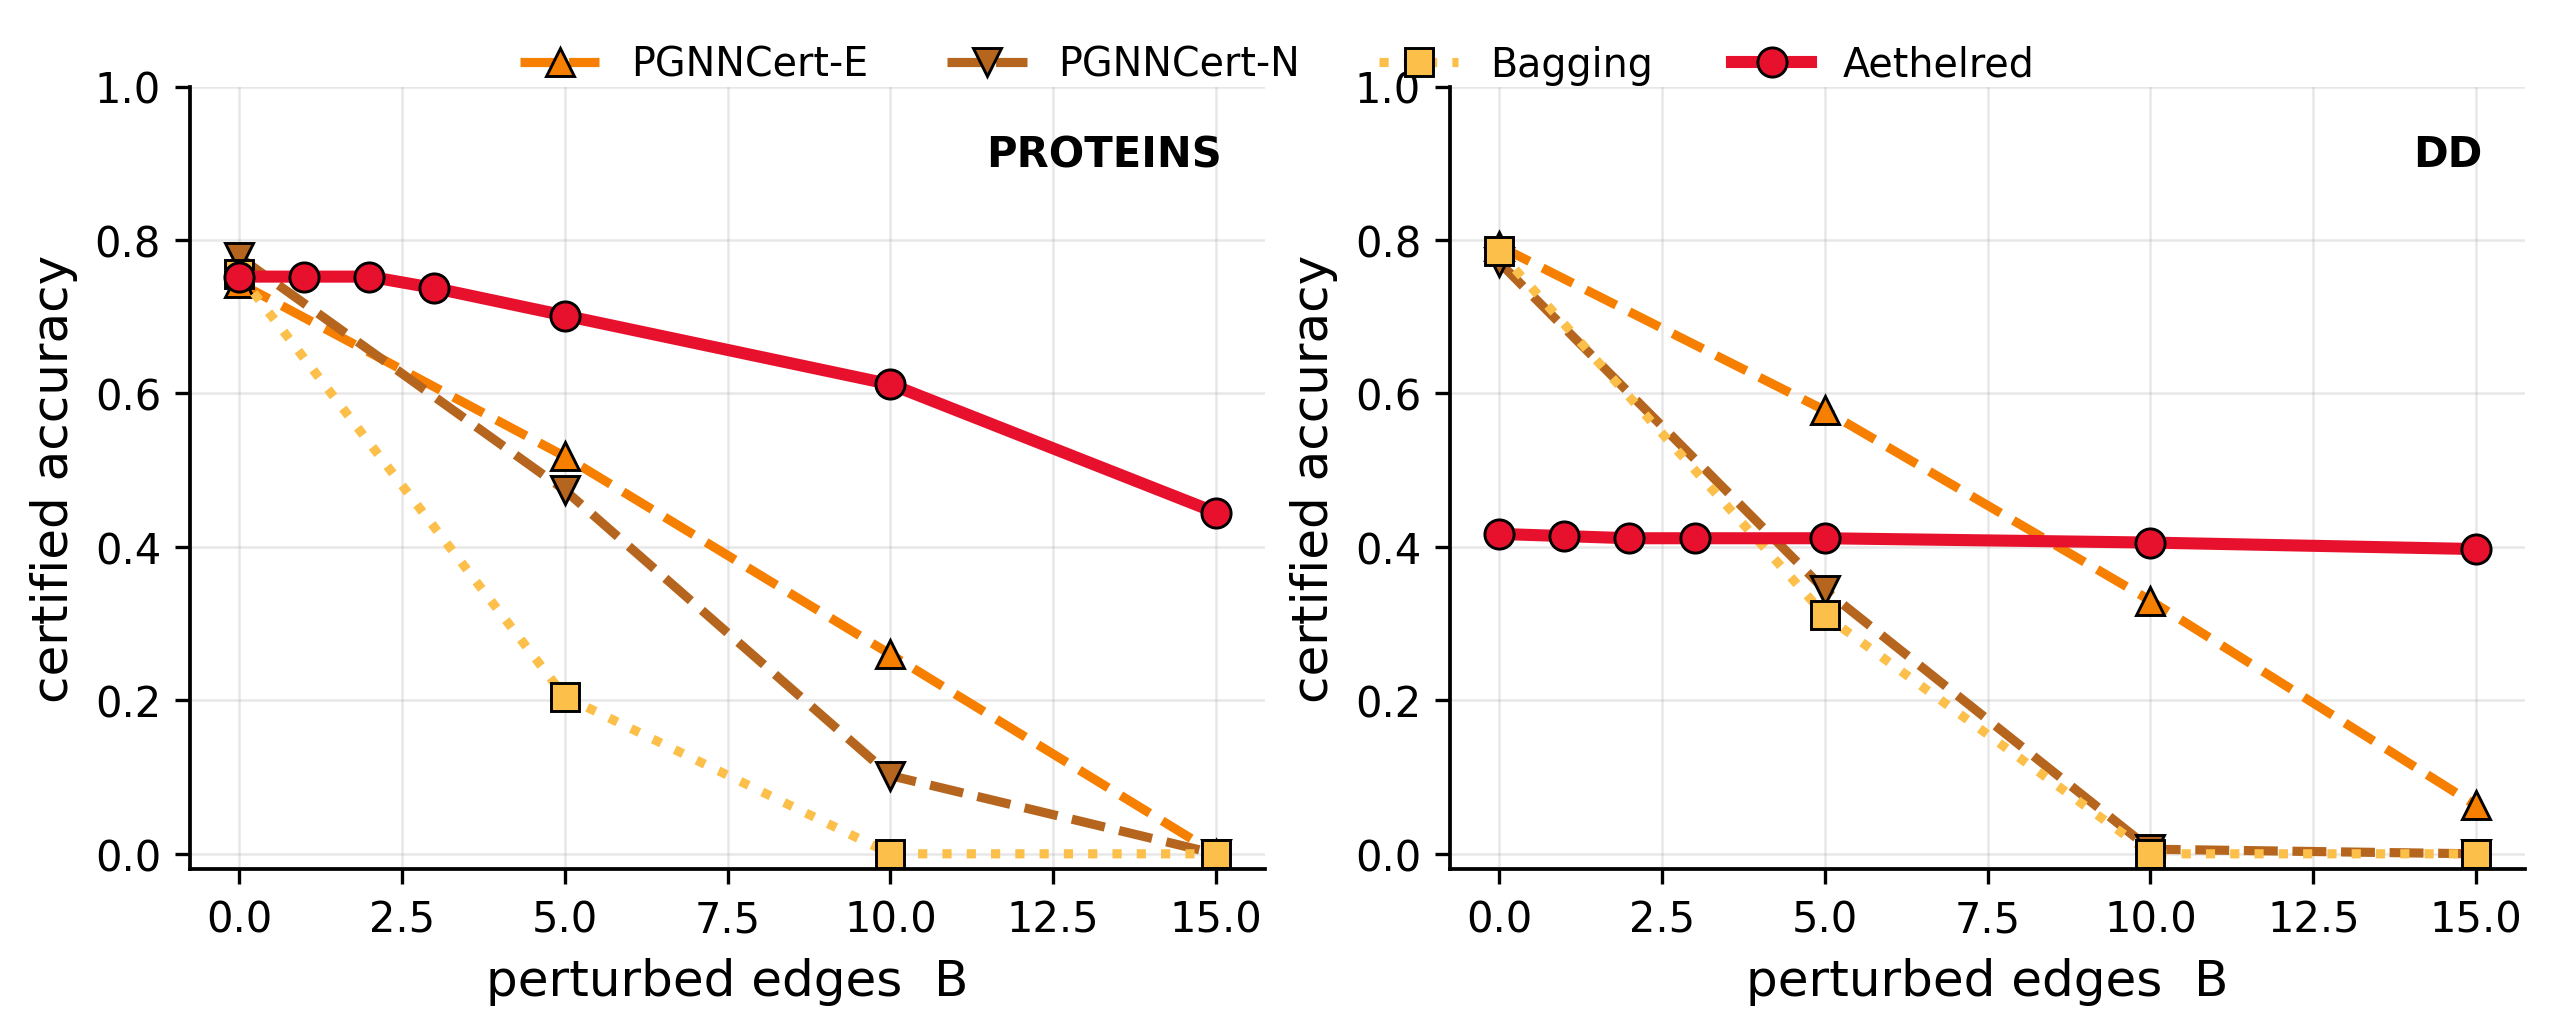
\includegraphics[width=\linewidth]{../../figures/F1_certified_prediction_vs_budget.png}
  \caption{Certified \emph{prediction} accuracy vs.\ edge budget (secondary
  axis), PROTEINS/DD; baselines from \pgn{}'s Table~2.}
  \label{fig:predcert}
\end{figure}

\begin{figure}[t]\centering
  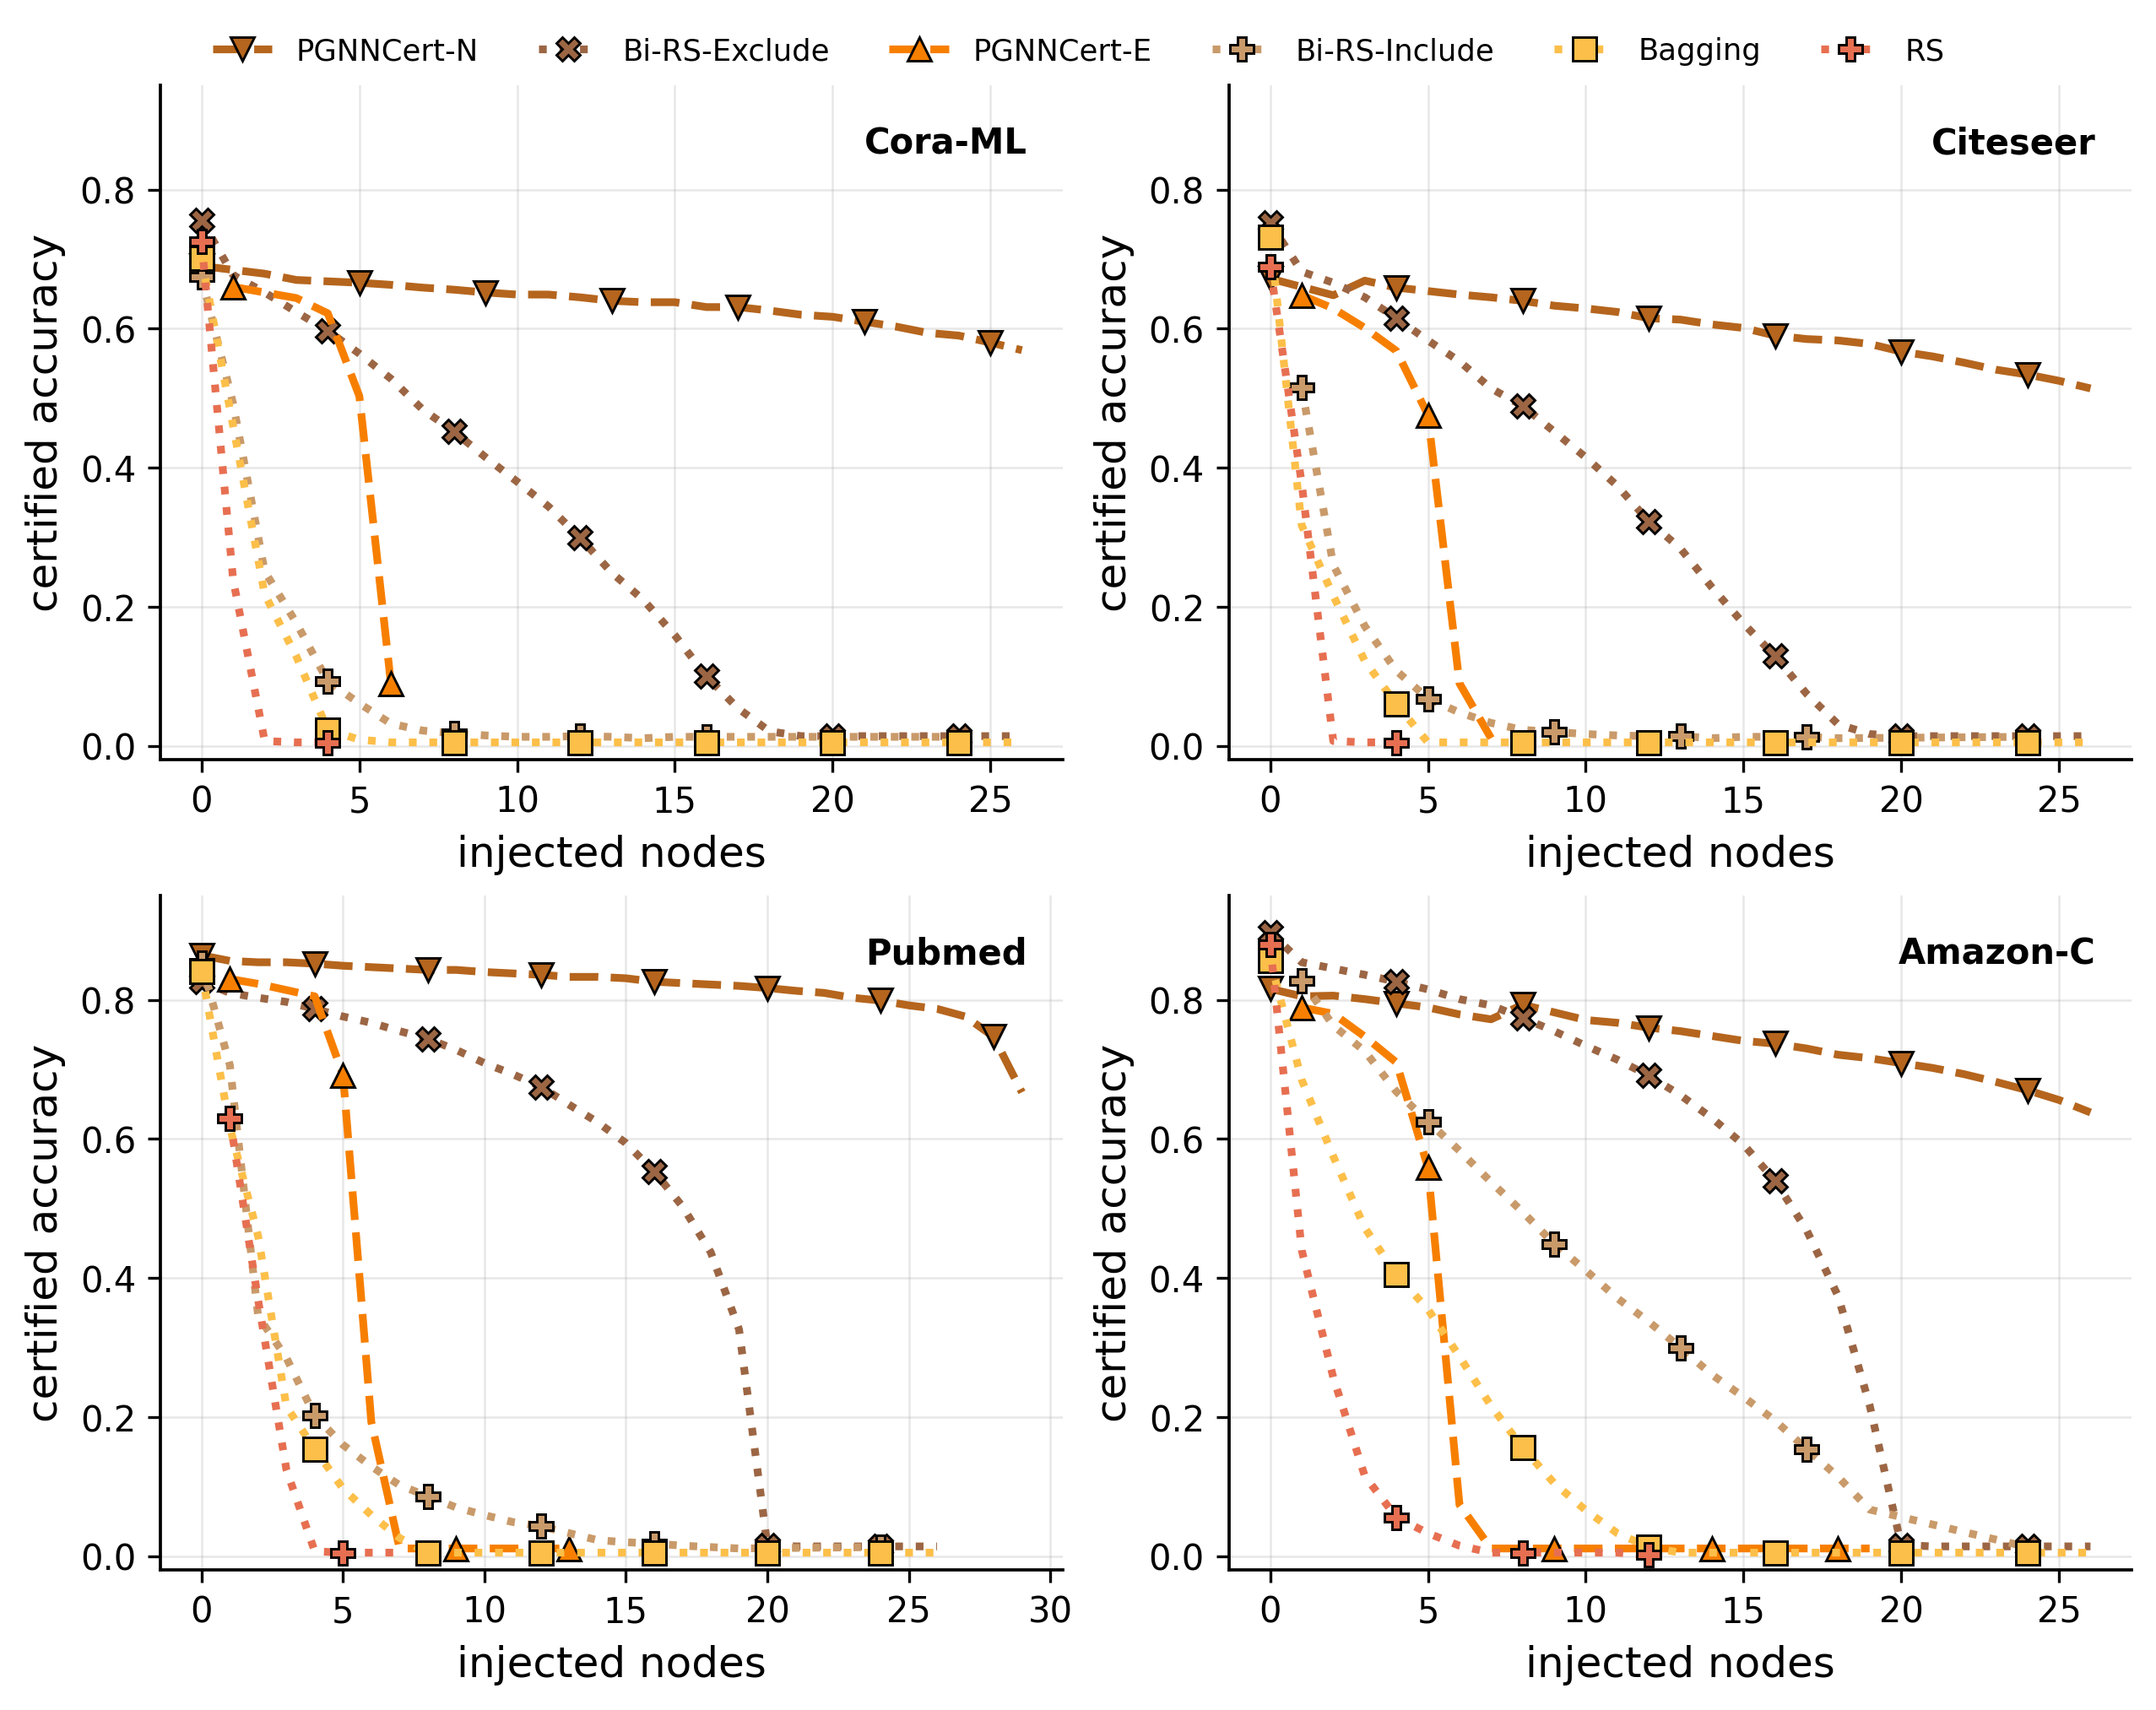
\includegraphics[width=\linewidth]{../../figures/F1b_node_injection_sota.png}
  \caption{Node-injection certified robustness across node datasets---a distinct
  threat model (node classification) shown as field context; \aeth{} targets
  graph-explanation edges.}
  \label{fig:nodeinj}
\end{figure}

\begin{table}[t]\centering
  \caption{Clean accuracy (5 seeds), \aeth{} vs.\ a plain GNN at the baseline's
  learning rate.}
  \label{tab:cleanacc}
  \begin{tabular}{lccc}
    \toprule
    Dataset & Base-GCN & \aeth{}-GCN & $\Delta$ \\
    \midrule
    AIDS & 0.986 & 0.989 & \win{$+0.3$} \\
    MUTAG & 0.762 & 0.769 & \win{$+0.7$} \\
    PROTEINS & 0.740 & 0.764 & \win{$+2.4$} \\
    DD & 0.725 & 0.758 & \win{$+3.4$} \\
    \midrule
    Cora-ML & 0.766 & 0.774 & $+0.8$ \\
    CiteSeer & 0.739 & 0.721 & \cav{$-1.7$} \\
    PubMed & 0.867 & 0.863 & $-0.4$ \\
    Amazon-C & 0.883 & 0.879 & $-0.3$ \\
    \bottomrule
  \end{tabular}
\end{table}



% =====================================================================
\section{Conclusion}
\label{sec:concl}
We argued that certifying the \emph{stability} of a GNN explanation is
insufficient---a stable explanation can be spurious---and introduced \aeth{},
which certifies the robustness of \emph{causally faithful} explanations with a
deterministic, tight, single-pass certificate. The certificate follows from a
propagation-free causal scorer whose edge-locality we exploit in closed form. On
the state of the art's own metric and published numbers \aeth{} certifies
markedly larger perturbation sizes on real data, remains faithful under spurious
correlation, and certifies at $\bigO(1)$ cost. We hope this reframes certified
explainability around \emph{what} is certified, not only \emph{how robustly}.

% =====================================================================
\bibliographystyle{aaai2026}   % <-- official AAAI .bst goes alongside the .sty
\bibliography{refs}

% =====================================================================
\appendix
% =====================================================================
%  Technical appendix: full proofs of the deterministic edge certificate.
%  \input by main.tex after the bibliography. Restated results are kept
%  UNNUMBERED (bold) so the body's Prop.~1 / Thm.~1--3 numbering is intact.
% =====================================================================

\section{Proofs of the Edge Certificate}
\label{app:proofs}

Throughout, an explanation is the set $\Ek=\{e_1,\dots,e_k\}$ of the $k$
highest-scoring \emph{undirected} edges of the clean graph, ordered
$s(e_1)\ge\cdots\ge s(e_M)$. An adversary applies a perturbation
$\pi=(\mathcal{A},\mathcal{D})$: a set $\mathcal{A}$ of added edges and a set
$\mathcal{D}$ of deleted edges, with total budget
$|\mathcal{A}|+|\mathcal{D}|\le B$. Let $G'$ be the perturbed graph and
$\Ek'$ its top-$k$ explanation. All scores are taken from the Causal Discovery
Core, $s(u,v)=\sigma(\mathrm{MLP}[\,h_u,h_v,|h_u-h_v|,\cos(x_u,x_v)\,])$ with
$h_u=\mathrm{MLP}(x_u)$.

\paragraph{Undirected aggregation.}
The core scores directed edges; \aeth{} stores each physical edge as the pair
$(u,v),(v,u)$ and the unit of perturbation is the \emph{physical} (undirected)
edge. We assign each physical edge the mean of its two directed scores,
$s(\{u,v\})=\tfrac12\big(s(u,v)+s(v,u)\big)$. Because each directed score is a
function of its own two endpoints' features only, $s(\{u,v\})$ is a function of
$\{x_u,x_v\}$ only; adding or deleting any \emph{other} physical edge leaves it
unchanged. This is the sole property the proofs use.

\subsection*{Proposition~\ref{prop:local} (Edge-locality), restated}
\emph{For any perturbation that adds or deletes edges other than $e$, the score
$s(e)$ is unchanged.}

\begin{proof}
$s(e)$ depends only on the features of $e$'s two endpoints (above). Edge
additions and deletions do not alter node features, and the node set is fixed
(both threat models in \xgn{}/\pgn{} perturb $E$, not $X$ or $V$). Hence any
$\pi$ that does not itself add or delete $e$ leaves the features of $e$'s
endpoints---and therefore $s(e)$---invariant.
\end{proof}

A first corollary, used repeatedly: \emph{deletions of edges other than $e$
leave both $s(e)$ and the entire relative ranking of all surviving edges
unchanged}, since every surviving score is individually invariant and ranking
depends only on the multiset of scores.

\subsection*{Theorem~\ref{thm:overlap} (Certified overlap), restated}
\emph{For any $\pi$ with $|\mathcal{A}|+|\mathcal{D}|\le B$,
$\;|\Ek\cap\Ek'|\ge k-B$.}

\begin{proof}
We bound the number of clean explanatory edges that can leave the top-$k$. An
edge $e_i\in\Ek$ can fail to lie in $\Ek'$ in exactly two ways.

\emph{(i) Direct deletion.} If $e_i\in\mathcal{D}$, it is absent from $G'$ and
hence from $\Ek'$. Each deletion removes at most one member of $\Ek$, so
deletions account for at most $|\mathcal{D}|$ losses.

\emph{(ii) Eviction by an addition.} Suppose $e_i\notin\mathcal{D}$. By
Prop.~\ref{prop:local} its score $s(e_i)$ and the scores of all other surviving
clean edges are unchanged, so among the surviving clean edges the ranking is
identical to the clean ranking. The only edges that can outrank $e_i$ in $G'$
beyond those that already did are the added edges $\mathcal{A}$. Each added edge
occupies exactly one position in the sorted order of $G'$; thus the $a$ added
edges collectively push the clean edges down by at most $a$ positions in total,
and---because each added edge sits in a single slot---can displace at most
$|\mathcal{A}|$ clean edges out of the top-$k$. Formally, the number of clean
survivors with final rank $>k$ is at most the number of added edges with score
exceeding the clean $k$-th score, which is at most $|\mathcal{A}|$.

Combining, the number of members of $\Ek$ absent from $\Ek'$ is at most
$|\mathcal{D}|+|\mathcal{A}|\le B$. Therefore
$|\Ek\cap\Ek'|\ge k-B$.
\end{proof}

\subsection*{Theorem~\ref{thm:radius} (Per-edge certified radius), restated}
\emph{The rank-$r$ edge $e_r\in\Ek$ (with $r\le k$) remains in the top-$k$
explanation under any $\pi$ with $|\mathcal{A}|+|\mathcal{D}|\le R(e_r)=k-r$ that
does not delete $e_r$.}

\begin{proof}
Assume $e_r\notin\mathcal{D}$. By Prop.~\ref{prop:local}, $s(e_r)$ is unchanged
and every surviving clean edge keeps its score, so in $G'$ the only edges that
can be ranked above $e_r$ are (a) the $r-1$ clean edges already above it and (b)
those added edges whose score exceeds $s(e_r)$. Deletions of other edges only
remove competitors, weakly improving $e_r$'s rank. Writing $a\le|\mathcal{A}|$
for the number of added edges scoring above $s(e_r)$, the rank of $e_r$ in $G'$
is at most $r+a$. Hence $e_r$ stays in the top-$k$ whenever $r+a\le k$, i.e.\
whenever $a\le k-r$. Since $a\le|\mathcal{A}|\le B$, a budget $B\le k-r$
suffices, giving the certified radius $R(e_r)=k-r$.
\end{proof}

\noindent\textbf{Remark (consistency with Thm.~\ref{thm:overlap}).} Summing the
per-edge radii recovers the overlap bound: the $j$-th-from-bottom member of
$\Ek$ has rank $r=k-j+1$ and radius $j-1$, so it can be evicted only once the
budget exceeds $j-1$; at budget $B$ at most the bottom $B$ members are at risk,
again yielding $|\Ek\cap\Ek'|\ge k-B$.

\subsection*{Theorem~\ref{thm:hijack} (Transductive hijack impossibility), restated}
\emph{In the transductive setting, let the structural-prior allowlist be active
with cap $c<1$, so every edge outside the training adjacency has score at most
$c$. If every $e_i\in\Ek$ has clean score $s(e_i)>c$, then no inserted edge can
enter $\Ek'$, for any budget $B$; the explanation can lose members only by
direct deletion.}

\begin{proof}
Every added edge is, by construction, absent from the training adjacency, so the
allowlist multiplier caps its score at $c$. By hypothesis $s(e_i)>c$ for all
$e_i\in\Ek$, hence every added edge scores strictly below every clean
explanatory edge. In the proof of Thm.~\ref{thm:radius}, the count $a$ of added
edges outranking a member $e_i$ is therefore $0$ regardless of $|\mathcal{A}|$:
the certified radius against additions is $R(e_i)=\infty$. Consequently no added
edge ever occupies a top-$k$ slot, and the only way to reduce $|\Ek\cap\Ek'|$ is
to delete clean members directly. The attacker-\emph{insertion} (hijack) rate is
thus exactly $0$ for unbounded $B$.
\end{proof}

This guarantee has no analogue for voting-based certificates: a smoothing/voting
explainer can always be hijacked with enough budget because an inserted edge
participates in (and can flip the vote of) many sub-graphs. The empirical check
agrees---$18/18$ top-$k$ edges survive $B=100$ insertions.

\subsection*{Tightness}
The overlap bound is achieved with equality, so no sound certificate of this
form can be larger. Fix $B\le k$. Construct an adversary that adds $B$ edges
whose endpoint features yield scores above $s(e_k)$ (e.g.\ duplicating the
endpoint profile of $e_1$). By the eviction argument these displace exactly the
$B$ lowest-ranked members of $\Ek$, giving $|\Ek\cap\Ek'|=k-B$. Hence the bound
of Thm.~\ref{thm:overlap} is tight, the certified--empirical gap is $0$, and the
greedy adversary of Fig.~\ref{fig:tight} realizes it---in contrast to randomized
smoothing, whose lower bound is strictly below the worst case it admits.

\subsection*{Soundness gate}
Because the certificate is deterministic, soundness is checkable exactly. For
each trained model and dataset we run the worst-case adversary of the tightness
construction at every budget $B$ and confirm the \emph{realized} overlap never
falls below $k-B$ (function \texttt{soundness\_check}). This gate must pass
before any large certification sweep; an unsound certificate would otherwise
invalidate every downstream number. All reported configurations pass with the
gap closing exactly at the bound.


\end{document}
